\documentclass[twoside]{book}

% Packages required by doxygen
\usepackage{fixltx2e}
\usepackage{calc}
\usepackage{doxygen}
\usepackage[export]{adjustbox} % also loads graphicx
\usepackage{graphicx}
\usepackage[utf8]{inputenc}
\usepackage{makeidx}
\usepackage{multicol}
\usepackage{multirow}
\PassOptionsToPackage{warn}{textcomp}
\usepackage{textcomp}
\usepackage[nointegrals]{wasysym}
\usepackage[table]{xcolor}

% Font selection
\usepackage[T1]{fontenc}
\usepackage[scaled=.90]{helvet}
\usepackage{courier}
\usepackage{amssymb}
\usepackage{sectsty}
\renewcommand{\familydefault}{\sfdefault}
\allsectionsfont{%
  \fontseries{bc}\selectfont%
  \color{darkgray}%
}
\renewcommand{\DoxyLabelFont}{%
  \fontseries{bc}\selectfont%
  \color{darkgray}%
}
\newcommand{\+}{\discretionary{\mbox{\scriptsize$\hookleftarrow$}}{}{}}

% Page & text layout
\usepackage{geometry}
\geometry{%
  a4paper,%
  top=2.5cm,%
  bottom=2.5cm,%
  left=2.5cm,%
  right=2.5cm%
}
\tolerance=750
\hfuzz=15pt
\hbadness=750
\setlength{\emergencystretch}{15pt}
\setlength{\parindent}{0cm}
\setlength{\parskip}{3ex plus 2ex minus 2ex}
\makeatletter
\renewcommand{\paragraph}{%
  \@startsection{paragraph}{4}{0ex}{-1.0ex}{1.0ex}{%
    \normalfont\normalsize\bfseries\SS@parafont%
  }%
}
\renewcommand{\subparagraph}{%
  \@startsection{subparagraph}{5}{0ex}{-1.0ex}{1.0ex}{%
    \normalfont\normalsize\bfseries\SS@subparafont%
  }%
}
\makeatother

% Headers & footers
\usepackage{fancyhdr}
\pagestyle{fancyplain}
\fancyhead[LE]{\fancyplain{}{\bfseries\thepage}}
\fancyhead[CE]{\fancyplain{}{}}
\fancyhead[RE]{\fancyplain{}{\bfseries\leftmark}}
\fancyhead[LO]{\fancyplain{}{\bfseries\rightmark}}
\fancyhead[CO]{\fancyplain{}{}}
\fancyhead[RO]{\fancyplain{}{\bfseries\thepage}}
\fancyfoot[LE]{\fancyplain{}{}}
\fancyfoot[CE]{\fancyplain{}{}}
\fancyfoot[RE]{\fancyplain{}{\bfseries\scriptsize Generated by Doxygen }}
\fancyfoot[LO]{\fancyplain{}{\bfseries\scriptsize Generated by Doxygen }}
\fancyfoot[CO]{\fancyplain{}{}}
\fancyfoot[RO]{\fancyplain{}{}}
\renewcommand{\footrulewidth}{0.4pt}
\renewcommand{\chaptermark}[1]{%
  \markboth{#1}{}%
}
\renewcommand{\sectionmark}[1]{%
  \markright{\thesection\ #1}%
}

% Indices & bibliography
\usepackage{natbib}
\usepackage[titles]{tocloft}
\setcounter{tocdepth}{3}
\setcounter{secnumdepth}{5}
\makeindex

% Hyperlinks (required, but should be loaded last)
\usepackage{ifpdf}
\ifpdf
  \usepackage[pdftex,pagebackref=true]{hyperref}
\else
  \usepackage[ps2pdf,pagebackref=true]{hyperref}
\fi
\hypersetup{%
  colorlinks=true,%
  linkcolor=blue,%
  citecolor=blue,%
  unicode%
}

% Custom commands
\newcommand{\clearemptydoublepage}{%
  \newpage{\pagestyle{empty}\cleardoublepage}%
}

\usepackage{caption}
\captionsetup{labelsep=space,justification=centering,font={bf},singlelinecheck=off,skip=4pt,position=top}

%===== C O N T E N T S =====

\begin{document}

% Titlepage & ToC
\hypersetup{pageanchor=false,
             bookmarksnumbered=true,
             pdfencoding=unicode
            }
\pagenumbering{alph}
\begin{titlepage}
\vspace*{7cm}
\begin{center}%
{\Large Elevator Project }\\
\vspace*{1cm}
{\large Generated by Doxygen 1.8.13}\\
\end{center}
\end{titlepage}
\clearemptydoublepage
\pagenumbering{roman}
\tableofcontents
\clearemptydoublepage
\pagenumbering{arabic}
\hypersetup{pageanchor=true}

%--- Begin generated contents ---
\chapter{Data Structure Index}
\section{Data Structures}
Here are the data structures with brief descriptions\+:\begin{DoxyCompactList}
\item\contentsline{section}{\hyperlink{structElevator}{Elevator} \\*An \hyperlink{structElevator}{Elevator} struct which holds a queue system, memory variables and control variables }{\pageref{structElevator}}{}
\end{DoxyCompactList}

\chapter{File Index}
\section{File List}
Here is a list of all documented files with brief descriptions\+:\begin{DoxyCompactList}
\item\contentsline{section}{source/{\bfseries elevator.\+c} }{\pageref{elevator_8c}}{}
\item\contentsline{section}{source/\hyperlink{elevator_8h}{elevator.\+h} \\*Library for an \hyperlink{structElevator}{Elevator} struct, and for operations on an \hyperlink{structElevator}{Elevator} struct }{\pageref{elevator_8h}}{}
\item\contentsline{section}{source/\hyperlink{hardware_8h}{hardware.\+h} \\*Driver for the elevator hardware }{\pageref{hardware_8h}}{}
\item\contentsline{section}{source/{\bfseries main.\+c} }{\pageref{main_8c}}{}
\item\contentsline{section}{source/{\bfseries queue\+\_\+handler.\+c} }{\pageref{queue__handler_8c}}{}
\item\contentsline{section}{source/\hyperlink{queue__handler_8h}{queue\+\_\+handler.\+h} \\*Library for doing operations with a queue matrix defined in an \hyperlink{structElevator}{Elevator} struct }{\pageref{queue__handler_8h}}{}
\item\contentsline{section}{source/{\bfseries states.\+c} }{\pageref{states_8c}}{}
\item\contentsline{section}{source/\hyperlink{states_8h}{states.\+h} \\*Library containing the state enum }{\pageref{states_8h}}{}
\item\contentsline{section}{source/{\bfseries stop\+\_\+btn.\+c} }{\pageref{stop__btn_8c}}{}
\item\contentsline{section}{source/\hyperlink{stop__btn_8h}{stop\+\_\+btn.\+h} \\*Library for stop button operations }{\pageref{stop__btn_8h}}{}
\item\contentsline{section}{source/{\bfseries timer.\+c} }{\pageref{timer_8c}}{}
\item\contentsline{section}{source/\hyperlink{timer_8h}{timer.\+h} \\*Library for timer operations }{\pageref{timer_8h}}{}
\item\contentsline{section}{source/{\bfseries utilities.\+c} }{\pageref{utilities_8c}}{}
\item\contentsline{section}{source/\hyperlink{utilities_8h}{utilities.\+h} \\*Useful functions }{\pageref{utilities_8h}}{}
\end{DoxyCompactList}

\chapter{Data Structure Documentation}
\hypertarget{structElevator}{}\doxysection{Elevator Struct Reference}
\label{structElevator}\index{Elevator@{Elevator}}


An \mbox{\hyperlink{structElevator}{Elevator}} struct which holds a queue system, memory variables and control variables.  




{\ttfamily \#include $<$elevator.\+h$>$}

\doxysubsection*{Data Fields}
\begin{DoxyCompactItemize}
\item 
\mbox{\Hypertarget{structElevator_ae9a4535426a6d35fed788c74685a3a1d}\label{structElevator_ae9a4535426a6d35fed788c74685a3a1d}} 
int {\bfseries queue\+\_\+matrix} \mbox{[}ELEVATOR\+\_\+\+NUMBER\+\_\+\+OF\+\_\+\+ORDERS\mbox{]}\mbox{[}HARDWARE\+\_\+\+NUMBER\+\_\+\+OF\+\_\+\+FLOORS\mbox{]}
\item 
\mbox{\Hypertarget{structElevator_aae297f56aca24d7be4518e2b14953015}\label{structElevator_aae297f56aca24d7be4518e2b14953015}} 
int {\bfseries current\+\_\+floor}
\item 
\mbox{\Hypertarget{structElevator_a4872eeb2a2737ff0396fca606f8eaad8}\label{structElevator_a4872eeb2a2737ff0396fca606f8eaad8}} 
int {\bfseries previous\+\_\+floor}
\item 
\mbox{\Hypertarget{structElevator_a787e17e94bf318d8757bbdf7ba0c7533}\label{structElevator_a787e17e94bf318d8757bbdf7ba0c7533}} 
\mbox{\hyperlink{hardware_8h_a2167c399a24df296afc432bcb88228af}{Hardware\+Movement}} {\bfseries current\+\_\+movement}
\item 
\mbox{\Hypertarget{structElevator_a4fb7d656caf15d55bdb47a603c43054e}\label{structElevator_a4fb7d656caf15d55bdb47a603c43054e}} 
\mbox{\hyperlink{hardware_8h_a2167c399a24df296afc432bcb88228af}{Hardware\+Movement}} {\bfseries previous\+\_\+direction}
\item 
\mbox{\Hypertarget{structElevator_ae20f4287465b4f67528853bebd3d3896}\label{structElevator_ae20f4287465b4f67528853bebd3d3896}} 
\mbox{\hyperlink{hardware_8h_a796a8de8ce0ae769d7dbd3327a7bdbe7}{Hardware\+Order}} {\bfseries order\+\_\+direction}
\item 
\mbox{\Hypertarget{structElevator_ad09af9fded96d746e098af616a052ade}\label{structElevator_ad09af9fded96d746e098af616a052ade}} 
\mbox{\hyperlink{states_8h_adc6e5733fc3c22f0a7b2914188c49c90}{state}} {\bfseries current\+\_\+state}
\item 
\mbox{\Hypertarget{structElevator_a6f567852f3f96cc1a7d1fc15aa4c0ad8}\label{structElevator_a6f567852f3f96cc1a7d1fc15aa4c0ad8}} 
int {\bfseries stop\+\_\+light\+\_\+set}
\item 
\mbox{\Hypertarget{structElevator_ab473c517dd118bdfd83928ec9afc9408}\label{structElevator_ab473c517dd118bdfd83928ec9afc9408}} 
int {\bfseries timer\+\_\+set}
\end{DoxyCompactItemize}


\doxysubsection{Detailed Description}
An \mbox{\hyperlink{structElevator}{Elevator}} struct which holds a queue system, memory variables and control variables. 


\begin{DoxyParams}{Parameters}
{\em queue\+\_\+matrix} & A matrix that holds a value for every type of order at every floor for the elevator. The values are non-\/zero for an active order and zero for a none-\/active order \\
\hline
{\em current\+\_\+floor} & Holds the value for the current or last visited floor \\
\hline
{\em previous\+\_\+floor} & Holds the value for the previously visited floor \\
\hline
{\em current\+\_\+movement} & Holds the value for the current direction of the elevator \\
\hline
{\em previous\+\_\+direction} & Holds the value for the previous direction of the elevator \\
\hline
{\em order\+\_\+direction} & Holds the value for the order type of the last handled order \\
\hline
{\em current\+\_\+state} & Holds the current state for the elevator \\
\hline
{\em stop\+\_\+light\+\_\+set} & A truthy value for if the stop light is set \\
\hline
{\em timer\+\_\+set} & A truthy value for if the timer has been set \\
\hline
\end{DoxyParams}


Definition at line 30 of file elevator.\+h.



The documentation for this struct was generated from the following file\+:\begin{DoxyCompactItemize}
\item 
source/\mbox{\hyperlink{elevator_8h}{elevator.\+h}}\end{DoxyCompactItemize}

\chapter{File Documentation}
\hypertarget{channels_8h}{}\section{source/driver/channels.h File Reference}
\label{channels_8h}\index{source/driver/channels.\+h@{source/driver/channels.\+h}}


Channel definitions for elevator control using Lib\+Comedi.  


This graph shows which files directly or indirectly include this file\+:
\nopagebreak
\begin{figure}[H]
\begin{center}
\leavevmode
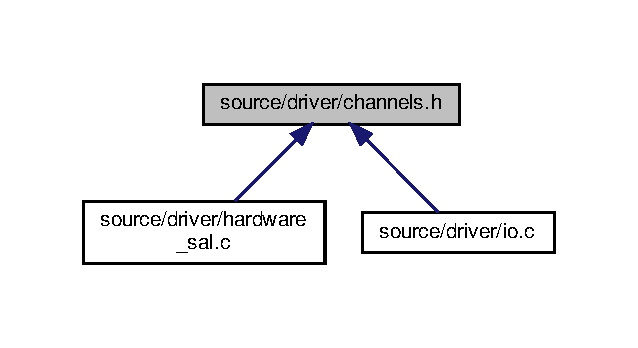
\includegraphics[width=306pt]{channels_8h__dep__incl}
\end{center}
\end{figure}
\subsection*{Macros}
\begin{DoxyCompactItemize}
\item 
\mbox{\Hypertarget{channels_8h_ad5a54f368997d8ae4f84a1e2fad533f4}\label{channels_8h_ad5a54f368997d8ae4f84a1e2fad533f4}} 
\#define {\bfseries P\+O\+R\+T4}~3
\item 
\mbox{\Hypertarget{channels_8h_a2409f02d98d288f64712887bd13b853e}\label{channels_8h_a2409f02d98d288f64712887bd13b853e}} 
\#define {\bfseries O\+B\+S\+T\+R\+U\+C\+T\+I\+ON}~(0x300+23)
\item 
\mbox{\Hypertarget{channels_8h_ae19b6bb2940d2fbe0a79852b070eeafd}\label{channels_8h_ae19b6bb2940d2fbe0a79852b070eeafd}} 
\#define {\bfseries S\+T\+OP}~(0x300+22)
\item 
\mbox{\Hypertarget{channels_8h_a1a22e01173ae543c7350d23af9099083}\label{channels_8h_a1a22e01173ae543c7350d23af9099083}} 
\#define {\bfseries B\+U\+T\+T\+O\+N\+\_\+\+C\+O\+M\+M\+A\+N\+D1}~(0x300+21)
\item 
\mbox{\Hypertarget{channels_8h_a8f3d02fddfb1ecd5227eca135f19ebd6}\label{channels_8h_a8f3d02fddfb1ecd5227eca135f19ebd6}} 
\#define {\bfseries B\+U\+T\+T\+O\+N\+\_\+\+C\+O\+M\+M\+A\+N\+D2}~(0x300+20)
\item 
\mbox{\Hypertarget{channels_8h_a82aab21b1b50d554effcf8b26576b388}\label{channels_8h_a82aab21b1b50d554effcf8b26576b388}} 
\#define {\bfseries B\+U\+T\+T\+O\+N\+\_\+\+C\+O\+M\+M\+A\+N\+D3}~(0x300+19)
\item 
\mbox{\Hypertarget{channels_8h_add9ae7df96dfd4ad569d3b703023187d}\label{channels_8h_add9ae7df96dfd4ad569d3b703023187d}} 
\#define {\bfseries B\+U\+T\+T\+O\+N\+\_\+\+C\+O\+M\+M\+A\+N\+D4}~(0x300+18)
\item 
\mbox{\Hypertarget{channels_8h_a7236f6ea90139248afabe014632c3cec}\label{channels_8h_a7236f6ea90139248afabe014632c3cec}} 
\#define {\bfseries B\+U\+T\+T\+O\+N\+\_\+\+U\+P1}~(0x300+17)
\item 
\mbox{\Hypertarget{channels_8h_a3a95d31cf2002937c921bbd85590bc7a}\label{channels_8h_a3a95d31cf2002937c921bbd85590bc7a}} 
\#define {\bfseries B\+U\+T\+T\+O\+N\+\_\+\+U\+P2}~(0x300+16)
\item 
\mbox{\Hypertarget{channels_8h_a83b698b796fa8d1625536439f28ea575}\label{channels_8h_a83b698b796fa8d1625536439f28ea575}} 
\#define {\bfseries P\+O\+R\+T1}~2
\item 
\mbox{\Hypertarget{channels_8h_a63a7b9d9d7c23325d4171292d596fa11}\label{channels_8h_a63a7b9d9d7c23325d4171292d596fa11}} 
\#define {\bfseries B\+U\+T\+T\+O\+N\+\_\+\+D\+O\+W\+N2}~(0x200+0)
\item 
\mbox{\Hypertarget{channels_8h_aa6b5917715e012cf21e3a89fb7c93e2d}\label{channels_8h_aa6b5917715e012cf21e3a89fb7c93e2d}} 
\#define {\bfseries B\+U\+T\+T\+O\+N\+\_\+\+U\+P3}~(0x200+1)
\item 
\mbox{\Hypertarget{channels_8h_ab423174da71ed0d6b083cd8d71f54617}\label{channels_8h_ab423174da71ed0d6b083cd8d71f54617}} 
\#define {\bfseries B\+U\+T\+T\+O\+N\+\_\+\+D\+O\+W\+N3}~(0x200+2)
\item 
\mbox{\Hypertarget{channels_8h_a7e1266fcb6843826718edec0222b1e49}\label{channels_8h_a7e1266fcb6843826718edec0222b1e49}} 
\#define {\bfseries B\+U\+T\+T\+O\+N\+\_\+\+D\+O\+W\+N4}~(0x200+3)
\item 
\mbox{\Hypertarget{channels_8h_a5ae95fe4e1273653467895d5e7c39377}\label{channels_8h_a5ae95fe4e1273653467895d5e7c39377}} 
\#define {\bfseries S\+E\+N\+S\+O\+R\+\_\+\+F\+L\+O\+O\+R1}~(0x200+4)
\item 
\mbox{\Hypertarget{channels_8h_ab9e1c393bf2c51d65ed0a132af8321d3}\label{channels_8h_ab9e1c393bf2c51d65ed0a132af8321d3}} 
\#define {\bfseries S\+E\+N\+S\+O\+R\+\_\+\+F\+L\+O\+O\+R2}~(0x200+5)
\item 
\mbox{\Hypertarget{channels_8h_a65904322d022513386fea3bcb9a8b524}\label{channels_8h_a65904322d022513386fea3bcb9a8b524}} 
\#define {\bfseries S\+E\+N\+S\+O\+R\+\_\+\+F\+L\+O\+O\+R3}~(0x200+6)
\item 
\mbox{\Hypertarget{channels_8h_a6a8d30abdce8780479ac7f0677200074}\label{channels_8h_a6a8d30abdce8780479ac7f0677200074}} 
\#define {\bfseries S\+E\+N\+S\+O\+R\+\_\+\+F\+L\+O\+O\+R4}~(0x200+7)
\item 
\mbox{\Hypertarget{channels_8h_ad906b7f6a811f1f02b5eb04cbe1bc89b}\label{channels_8h_ad906b7f6a811f1f02b5eb04cbe1bc89b}} 
\#define {\bfseries P\+O\+R\+T3}~3
\item 
\mbox{\Hypertarget{channels_8h_aaa316c7fc13ca7b9b4229af3f9832a7d}\label{channels_8h_aaa316c7fc13ca7b9b4229af3f9832a7d}} 
\#define {\bfseries M\+O\+T\+O\+R\+D\+IR}~(0x300+15)
\item 
\mbox{\Hypertarget{channels_8h_a7845eb8e4ab5e0a49739663d69ff9001}\label{channels_8h_a7845eb8e4ab5e0a49739663d69ff9001}} 
\#define {\bfseries L\+I\+G\+H\+T\+\_\+\+S\+T\+OP}~(0x300+14)
\item 
\mbox{\Hypertarget{channels_8h_a61e8bfbed9e1d63bbbce251b10b69d9b}\label{channels_8h_a61e8bfbed9e1d63bbbce251b10b69d9b}} 
\#define {\bfseries L\+I\+G\+H\+T\+\_\+\+C\+O\+M\+M\+A\+N\+D1}~(0x300+13)
\item 
\mbox{\Hypertarget{channels_8h_a05423733c25f39ca059f5bfae9e3fb33}\label{channels_8h_a05423733c25f39ca059f5bfae9e3fb33}} 
\#define {\bfseries L\+I\+G\+H\+T\+\_\+\+C\+O\+M\+M\+A\+N\+D2}~(0x300+12)
\item 
\mbox{\Hypertarget{channels_8h_aec8c2b567fd77cff4163ebab81b6abd1}\label{channels_8h_aec8c2b567fd77cff4163ebab81b6abd1}} 
\#define {\bfseries L\+I\+G\+H\+T\+\_\+\+C\+O\+M\+M\+A\+N\+D3}~(0x300+11)
\item 
\mbox{\Hypertarget{channels_8h_ad2ffefe386fcbad6a538f84c7fe191f3}\label{channels_8h_ad2ffefe386fcbad6a538f84c7fe191f3}} 
\#define {\bfseries L\+I\+G\+H\+T\+\_\+\+C\+O\+M\+M\+A\+N\+D4}~(0x300+10)
\item 
\mbox{\Hypertarget{channels_8h_aec0494e52bb28dfa15a8035c3359bd0f}\label{channels_8h_aec0494e52bb28dfa15a8035c3359bd0f}} 
\#define {\bfseries L\+I\+G\+H\+T\+\_\+\+U\+P1}~(0x300+9)
\item 
\mbox{\Hypertarget{channels_8h_ab4f192467448356764080a8102eb32f1}\label{channels_8h_ab4f192467448356764080a8102eb32f1}} 
\#define {\bfseries L\+I\+G\+H\+T\+\_\+\+U\+P2}~(0x300+8)
\item 
\mbox{\Hypertarget{channels_8h_acb270e4aec8a0ab123e6c24a5810150b}\label{channels_8h_acb270e4aec8a0ab123e6c24a5810150b}} 
\#define {\bfseries P\+O\+R\+T2}~3
\item 
\mbox{\Hypertarget{channels_8h_a919d92344f7934414150b99fe94d1ace}\label{channels_8h_a919d92344f7934414150b99fe94d1ace}} 
\#define {\bfseries L\+I\+G\+H\+T\+\_\+\+D\+O\+W\+N2}~(0x300+7)
\item 
\mbox{\Hypertarget{channels_8h_a2fd78cafe153eb500f5f6731f6a2d7c7}\label{channels_8h_a2fd78cafe153eb500f5f6731f6a2d7c7}} 
\#define {\bfseries L\+I\+G\+H\+T\+\_\+\+U\+P3}~(0x300+6)
\item 
\mbox{\Hypertarget{channels_8h_adc5182903fbf37402ed9a2b65af65a40}\label{channels_8h_adc5182903fbf37402ed9a2b65af65a40}} 
\#define {\bfseries L\+I\+G\+H\+T\+\_\+\+D\+O\+W\+N3}~(0x300+5)
\item 
\mbox{\Hypertarget{channels_8h_a1745b9fd720072a9ff8f58c75ca9512c}\label{channels_8h_a1745b9fd720072a9ff8f58c75ca9512c}} 
\#define {\bfseries L\+I\+G\+H\+T\+\_\+\+D\+O\+W\+N4}~(0x300+4)
\item 
\mbox{\Hypertarget{channels_8h_ab3e81b38bff9c0c8dd9dea97f3c42073}\label{channels_8h_ab3e81b38bff9c0c8dd9dea97f3c42073}} 
\#define {\bfseries L\+I\+G\+H\+T\+\_\+\+D\+O\+O\+R\+\_\+\+O\+P\+EN}~(0x300+3)
\item 
\mbox{\Hypertarget{channels_8h_a99e7a2989cfe5f085c49c31d033baae2}\label{channels_8h_a99e7a2989cfe5f085c49c31d033baae2}} 
\#define {\bfseries L\+I\+G\+H\+T\+\_\+\+F\+L\+O\+O\+R\+\_\+\+I\+N\+D2}~(0x300+1)
\item 
\mbox{\Hypertarget{channels_8h_a1b686be38adf6a919cceca00890df7c8}\label{channels_8h_a1b686be38adf6a919cceca00890df7c8}} 
\#define {\bfseries L\+I\+G\+H\+T\+\_\+\+F\+L\+O\+O\+R\+\_\+\+I\+N\+D1}~(0x300+0)
\item 
\mbox{\Hypertarget{channels_8h_af41b34488a518db05b413d3a370f871f}\label{channels_8h_af41b34488a518db05b413d3a370f871f}} 
\#define {\bfseries P\+O\+R\+T0}~1
\item 
\mbox{\Hypertarget{channels_8h_ae8d3b23b31729f61bc738fbd9a9a24e0}\label{channels_8h_ae8d3b23b31729f61bc738fbd9a9a24e0}} 
\#define {\bfseries M\+O\+T\+OR}~(0x100+0)
\item 
\mbox{\Hypertarget{channels_8h_a8bcc98057f83b3b335fa3d9865410d42}\label{channels_8h_a8bcc98057f83b3b335fa3d9865410d42}} 
\#define {\bfseries B\+U\+T\+T\+O\+N\+\_\+\+D\+O\+W\+N1}~-\/1
\item 
\mbox{\Hypertarget{channels_8h_a02cc4cce547c81453cf7b5e55dd24986}\label{channels_8h_a02cc4cce547c81453cf7b5e55dd24986}} 
\#define {\bfseries B\+U\+T\+T\+O\+N\+\_\+\+U\+P4}~-\/1
\item 
\mbox{\Hypertarget{channels_8h_ad63056bd0003fdef7bdf927bf2ff1118}\label{channels_8h_ad63056bd0003fdef7bdf927bf2ff1118}} 
\#define {\bfseries L\+I\+G\+H\+T\+\_\+\+D\+O\+W\+N1}~-\/1
\item 
\mbox{\Hypertarget{channels_8h_ab4e1e3be316a23e33d3080931737eb60}\label{channels_8h_ab4e1e3be316a23e33d3080931737eb60}} 
\#define {\bfseries L\+I\+G\+H\+T\+\_\+\+U\+P4}~-\/1
\end{DoxyCompactItemize}


\subsection{Detailed Description}
Channel definitions for elevator control using Lib\+Comedi. 


\hypertarget{io_8h}{}\doxysection{source/driver/io.h File Reference}
\label{io_8h}\index{source/driver/io.h@{source/driver/io.h}}


Wrapper for lib\+Comedi I/O These function provide and interface to lib\+Comedi limited to use in the real time lab.  


This graph shows which files directly or indirectly include this file\+:
% FIG 0
\doxysubsection*{Functions}
\begin{DoxyCompactItemize}
\item 
int \mbox{\hyperlink{io_8h_a12ce98b64f2019ac45b44826a4db7ec9}{io\+\_\+init}} ()
\item 
void \mbox{\hyperlink{io_8h_a4d538858b80ee856217e3ecfde8a3c60}{io\+\_\+set\+\_\+bit}} (int channel)
\item 
void \mbox{\hyperlink{io_8h_a97951257634a0778b858a4ced7558f81}{io\+\_\+clear\+\_\+bit}} (int channel)
\item 
void \mbox{\hyperlink{io_8h_a1c2c5df63111187109ef11be354621bd}{io\+\_\+write\+\_\+analog}} (int channel, int value)
\item 
int \mbox{\hyperlink{io_8h_ae9e08ee7d41b07b153e2ddaae4dc53cb}{io\+\_\+read\+\_\+bit}} (int channel)
\item 
int \mbox{\hyperlink{io_8h_ab145a5637d2c463dfb5741e1a748dd74}{io\+\_\+read\+\_\+analog}} (int channel)
\end{DoxyCompactItemize}


\doxysubsection{Detailed Description}
Wrapper for lib\+Comedi I/O These function provide and interface to lib\+Comedi limited to use in the real time lab. 



\doxysubsection{Function Documentation}
\mbox{\Hypertarget{io_8h_a97951257634a0778b858a4ced7558f81}\label{io_8h_a97951257634a0778b858a4ced7558f81}} 
\index{io.h@{io.h}!io\_clear\_bit@{io\_clear\_bit}}
\index{io\_clear\_bit@{io\_clear\_bit}!io.h@{io.h}}
\doxysubsubsection{\texorpdfstring{io\_clear\_bit()}{io\_clear\_bit()}}
{\footnotesize\ttfamily void io\+\_\+clear\+\_\+bit (\begin{DoxyParamCaption}\item[{int}]{channel }\end{DoxyParamCaption})}

Clears a digital channel bit. 
\begin{DoxyParams}{Parameters}
{\em channel} & Channel bit to set. \\
\hline
\end{DoxyParams}


Definition at line 45 of file io.\+c.

\mbox{\Hypertarget{io_8h_a12ce98b64f2019ac45b44826a4db7ec9}\label{io_8h_a12ce98b64f2019ac45b44826a4db7ec9}} 
\index{io.h@{io.h}!io\_init@{io\_init}}
\index{io\_init@{io\_init}!io.h@{io.h}}
\doxysubsubsection{\texorpdfstring{io\_init()}{io\_init()}}
{\footnotesize\ttfamily int io\+\_\+init (\begin{DoxyParamCaption}{ }\end{DoxyParamCaption})}

Initialize lib\+Comedi in \char`\"{}\+Sanntidssalen\char`\"{} \begin{DoxyReturn}{Returns}
Non-\/zero on success and 0 on failure 
\end{DoxyReturn}


Definition at line 18 of file io.\+c.

\mbox{\Hypertarget{io_8h_ab145a5637d2c463dfb5741e1a748dd74}\label{io_8h_ab145a5637d2c463dfb5741e1a748dd74}} 
\index{io.h@{io.h}!io\_read\_analog@{io\_read\_analog}}
\index{io\_read\_analog@{io\_read\_analog}!io.h@{io.h}}
\doxysubsubsection{\texorpdfstring{io\_read\_analog()}{io\_read\_analog()}}
{\footnotesize\ttfamily int io\+\_\+read\+\_\+analog (\begin{DoxyParamCaption}\item[{int}]{channel }\end{DoxyParamCaption})}

Reads a bit value from an analog channel. 
\begin{DoxyParams}{Parameters}
{\em channel} & Channel to read from. \\
\hline
\end{DoxyParams}
\begin{DoxyReturn}{Returns}
Value read. 
\end{DoxyReturn}


Definition at line 66 of file io.\+c.

\mbox{\Hypertarget{io_8h_ae9e08ee7d41b07b153e2ddaae4dc53cb}\label{io_8h_ae9e08ee7d41b07b153e2ddaae4dc53cb}} 
\index{io.h@{io.h}!io\_read\_bit@{io\_read\_bit}}
\index{io\_read\_bit@{io\_read\_bit}!io.h@{io.h}}
\doxysubsubsection{\texorpdfstring{io\_read\_bit()}{io\_read\_bit()}}
{\footnotesize\ttfamily int io\+\_\+read\+\_\+bit (\begin{DoxyParamCaption}\item[{int}]{channel }\end{DoxyParamCaption})}

Reads a bit value from a digital channel. 
\begin{DoxyParams}{Parameters}
{\em channel} & Channel to read from. \\
\hline
\end{DoxyParams}
\begin{DoxyReturn}{Returns}
Value read. 
\end{DoxyReturn}


Definition at line 57 of file io.\+c.

\mbox{\Hypertarget{io_8h_a4d538858b80ee856217e3ecfde8a3c60}\label{io_8h_a4d538858b80ee856217e3ecfde8a3c60}} 
\index{io.h@{io.h}!io\_set\_bit@{io\_set\_bit}}
\index{io\_set\_bit@{io\_set\_bit}!io.h@{io.h}}
\doxysubsubsection{\texorpdfstring{io\_set\_bit()}{io\_set\_bit()}}
{\footnotesize\ttfamily void io\+\_\+set\+\_\+bit (\begin{DoxyParamCaption}\item[{int}]{channel }\end{DoxyParamCaption})}

Sets a digital channel bit. 
\begin{DoxyParams}{Parameters}
{\em channel} & Channel bit to set. \\
\hline
\end{DoxyParams}


Definition at line 39 of file io.\+c.

\mbox{\Hypertarget{io_8h_a1c2c5df63111187109ef11be354621bd}\label{io_8h_a1c2c5df63111187109ef11be354621bd}} 
\index{io.h@{io.h}!io\_write\_analog@{io\_write\_analog}}
\index{io\_write\_analog@{io\_write\_analog}!io.h@{io.h}}
\doxysubsubsection{\texorpdfstring{io\_write\_analog()}{io\_write\_analog()}}
{\footnotesize\ttfamily void io\+\_\+write\+\_\+analog (\begin{DoxyParamCaption}\item[{int}]{channel,  }\item[{int}]{value }\end{DoxyParamCaption})}

Writes a value to an analog channel. 
\begin{DoxyParams}{Parameters}
{\em channel} & Channel to write to. \\
\hline
{\em value} & Value to write. \\
\hline
\end{DoxyParams}


Definition at line 51 of file io.\+c.


\hypertarget{elevator_8h}{}\doxysection{source/elevator.h File Reference}
\label{elevator_8h}\index{source/elevator.h@{source/elevator.h}}


Library for an \mbox{\hyperlink{structElevator}{Elevator}} struct, and for operations on an \mbox{\hyperlink{structElevator}{Elevator}} struct.  


{\ttfamily \#include $<$stdlib.\+h$>$}\newline
{\ttfamily \#include \char`\"{}utilities.\+h\char`\"{}}\newline
{\ttfamily \#include \char`\"{}states.\+h\char`\"{}}\newline
Include dependency graph for elevator.\+h\+:
\nopagebreak
\begin{figure}[H]
\begin{center}
\leavevmode
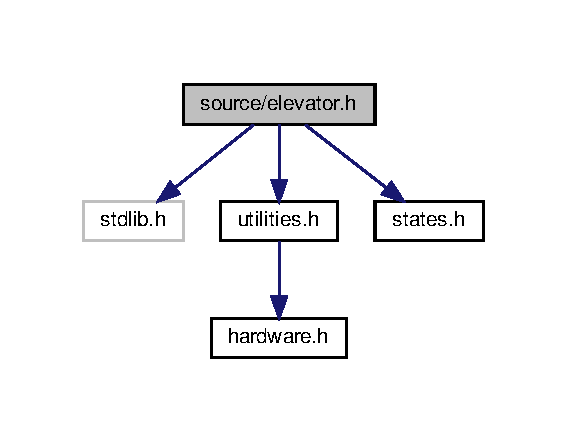
\includegraphics[width=272pt]{elevator_8h__incl}
\end{center}
\end{figure}
This graph shows which files directly or indirectly include this file\+:
\nopagebreak
\begin{figure}[H]
\begin{center}
\leavevmode
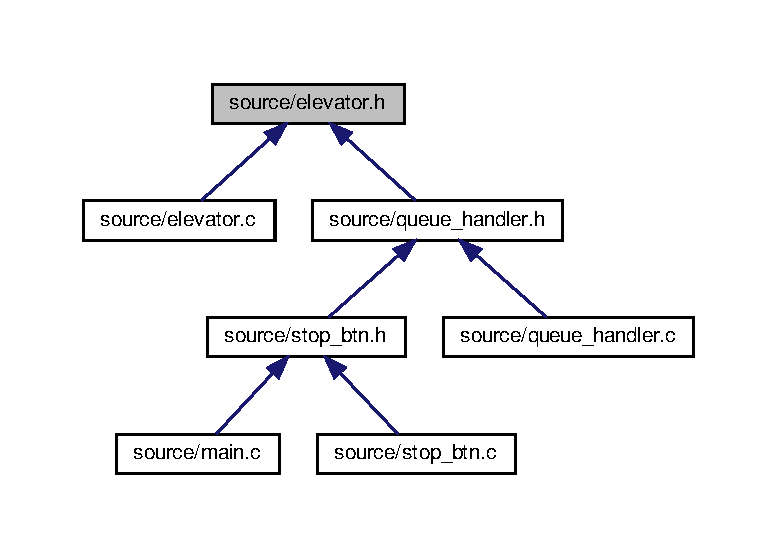
\includegraphics[width=350pt]{elevator_8h__dep__incl}
\end{center}
\end{figure}
\doxysubsection*{Data Structures}
\begin{DoxyCompactItemize}
\item 
struct \mbox{\hyperlink{structElevator}{Elevator}}
\begin{DoxyCompactList}\small\item\em An \mbox{\hyperlink{structElevator}{Elevator}} struct which holds a queue system, memory variables and control variables. \end{DoxyCompactList}\end{DoxyCompactItemize}
\doxysubsection*{Macros}
\begin{DoxyCompactItemize}
\item 
\mbox{\Hypertarget{elevator_8h_a5e9d3519138a42b79c6f8002347b7d88}\label{elevator_8h_a5e9d3519138a42b79c6f8002347b7d88}} 
\#define {\bfseries ELEVATOR\+\_\+\+NUMBER\+\_\+\+OF\+\_\+\+ORDERS}~3
\end{DoxyCompactItemize}
\doxysubsection*{Typedefs}
\begin{DoxyCompactItemize}
\item 
typedef struct \mbox{\hyperlink{structElevator}{Elevator}} \mbox{\hyperlink{elevator_8h_a9b4fd374e3626fffe1540f991c00f5c0}{Elevator}}
\begin{DoxyCompactList}\small\item\em An \mbox{\hyperlink{structElevator}{Elevator}} struct which holds a queue system, memory variables and control variables. \end{DoxyCompactList}\end{DoxyCompactItemize}
\doxysubsection*{Functions}
\begin{DoxyCompactItemize}
\item 
void \mbox{\hyperlink{elevator_8h_ad30b17a212bc32d6b2a9081c3ead4a3d}{elevator\+\_\+init}} (\mbox{\hyperlink{structElevator}{Elevator}} $\ast$p\+\_\+elev)
\begin{DoxyCompactList}\small\item\em Initialises the elements of {\ttfamily p\+\_\+elev} and sets queue\+\_\+matrix to a zero matrix. Sets current\+\_\+state to INIT. \end{DoxyCompactList}\item 
void \mbox{\hyperlink{elevator_8h_a7ab778bfdf149cd6f06b83c5102bbc79}{elevator\+\_\+startup\+\_\+routine}} (\mbox{\hyperlink{structElevator}{Elevator}} $\ast$p\+\_\+elev)
\begin{DoxyCompactList}\small\item\em Moves the elevator to a defined state and sets current\+\_\+movement, current\+\_\+direction and previous\+\_\+direction in {\ttfamily p\+\_\+elev}. Sets current\+\_\+state to IDLE\+\_\+\+IN\+\_\+\+FLOOR upon success. \end{DoxyCompactList}\item 
void \mbox{\hyperlink{elevator_8h_a006e863b777755b9d2ec96a78e620b28}{elevator\+\_\+order\+\_\+light\+\_\+on}} (\mbox{\hyperlink{structElevator}{Elevator}} $\ast$p\+\_\+elev)
\begin{DoxyCompactList}\small\item\em Sets the order lights for the order types and floors, in which {\ttfamily p\+\_\+elev} has active orders. \end{DoxyCompactList}\item 
void \mbox{\hyperlink{elevator_8h_a9b5f259e84b6ffed37e9c01709187c90}{elevator\+\_\+update\+\_\+floor}} (\mbox{\hyperlink{structElevator}{Elevator}} $\ast$p\+\_\+elev)
\begin{DoxyCompactList}\small\item\em Updates current\+\_\+floor and previous\+\_\+floor in {\ttfamily p\+\_\+elev} and sets the floor indicator. \end{DoxyCompactList}\end{DoxyCompactItemize}


\doxysubsection{Detailed Description}
Library for an \mbox{\hyperlink{structElevator}{Elevator}} struct, and for operations on an \mbox{\hyperlink{structElevator}{Elevator}} struct. 



\doxysubsection{Typedef Documentation}
\mbox{\Hypertarget{elevator_8h_a9b4fd374e3626fffe1540f991c00f5c0}\label{elevator_8h_a9b4fd374e3626fffe1540f991c00f5c0}} 
\index{elevator.h@{elevator.h}!Elevator@{Elevator}}
\index{Elevator@{Elevator}!elevator.h@{elevator.h}}
\doxysubsubsection{\texorpdfstring{Elevator}{Elevator}}
{\footnotesize\ttfamily typedef struct \mbox{\hyperlink{structElevator}{Elevator}} \mbox{\hyperlink{structElevator}{Elevator}}}



An \mbox{\hyperlink{structElevator}{Elevator}} struct which holds a queue system, memory variables and control variables. 


\begin{DoxyParams}{Parameters}
{\em queue\+\_\+matrix} & A matrix that holds a value for every type of order at every floor for the elevator. The values are non-\/zero for an active order and zero for a none-\/active order \\
\hline
{\em current\+\_\+floor} & Holds the value for the current or last visited floor \\
\hline
{\em previous\+\_\+floor} & Holds the value for the previously visited floor \\
\hline
{\em current\+\_\+movement} & Holds the value for the current direction of the elevator \\
\hline
{\em previous\+\_\+direction} & Holds the value for the previous direction of the elevator \\
\hline
{\em order\+\_\+direction} & Holds the value for the order type of the last handled order \\
\hline
{\em current\+\_\+state} & Holds the current state for the elevator \\
\hline
{\em stop\+\_\+light\+\_\+set} & A truthy value for if the stop light is set \\
\hline
{\em timer\+\_\+set} & A truthy value for if the timer has been set \\
\hline
\end{DoxyParams}


\doxysubsection{Function Documentation}
\mbox{\Hypertarget{elevator_8h_ad30b17a212bc32d6b2a9081c3ead4a3d}\label{elevator_8h_ad30b17a212bc32d6b2a9081c3ead4a3d}} 
\index{elevator.h@{elevator.h}!elevator\_init@{elevator\_init}}
\index{elevator\_init@{elevator\_init}!elevator.h@{elevator.h}}
\doxysubsubsection{\texorpdfstring{elevator\_init()}{elevator\_init()}}
{\footnotesize\ttfamily void elevator\+\_\+init (\begin{DoxyParamCaption}\item[{\mbox{\hyperlink{structElevator}{Elevator}} $\ast$}]{p\+\_\+elev }\end{DoxyParamCaption})}



Initialises the elements of {\ttfamily p\+\_\+elev} and sets queue\+\_\+matrix to a zero matrix. Sets current\+\_\+state to INIT. 


\begin{DoxyParams}[1]{Parameters}
\mbox{\texttt{ out}}  & {\em p\+\_\+elev} & Pointer to an \mbox{\hyperlink{structElevator}{Elevator}} struct \\
\hline
\end{DoxyParams}


Definition at line 3 of file elevator.\+c.

\mbox{\Hypertarget{elevator_8h_a006e863b777755b9d2ec96a78e620b28}\label{elevator_8h_a006e863b777755b9d2ec96a78e620b28}} 
\index{elevator.h@{elevator.h}!elevator\_order\_light\_on@{elevator\_order\_light\_on}}
\index{elevator\_order\_light\_on@{elevator\_order\_light\_on}!elevator.h@{elevator.h}}
\doxysubsubsection{\texorpdfstring{elevator\_order\_light\_on()}{elevator\_order\_light\_on()}}
{\footnotesize\ttfamily void elevator\+\_\+order\+\_\+light\+\_\+on (\begin{DoxyParamCaption}\item[{\mbox{\hyperlink{structElevator}{Elevator}} $\ast$}]{p\+\_\+elev }\end{DoxyParamCaption})}



Sets the order lights for the order types and floors, in which {\ttfamily p\+\_\+elev} has active orders. 


\begin{DoxyParams}[1]{Parameters}
\mbox{\texttt{ in}}  & {\em p\+\_\+elev} & Pointer to an \mbox{\hyperlink{structElevator}{Elevator}} struct \\
\hline
\end{DoxyParams}


Definition at line 32 of file elevator.\+c.

\mbox{\Hypertarget{elevator_8h_a7ab778bfdf149cd6f06b83c5102bbc79}\label{elevator_8h_a7ab778bfdf149cd6f06b83c5102bbc79}} 
\index{elevator.h@{elevator.h}!elevator\_startup\_routine@{elevator\_startup\_routine}}
\index{elevator\_startup\_routine@{elevator\_startup\_routine}!elevator.h@{elevator.h}}
\doxysubsubsection{\texorpdfstring{elevator\_startup\_routine()}{elevator\_startup\_routine()}}
{\footnotesize\ttfamily void elevator\+\_\+startup\+\_\+routine (\begin{DoxyParamCaption}\item[{\mbox{\hyperlink{structElevator}{Elevator}} $\ast$}]{p\+\_\+elev }\end{DoxyParamCaption})}



Moves the elevator to a defined state and sets current\+\_\+movement, current\+\_\+direction and previous\+\_\+direction in {\ttfamily p\+\_\+elev}. Sets current\+\_\+state to IDLE\+\_\+\+IN\+\_\+\+FLOOR upon success. 


\begin{DoxyParams}[1]{Parameters}
\mbox{\texttt{ out}}  & {\em p\+\_\+elev} & Pointer to an \mbox{\hyperlink{structElevator}{Elevator}} struct \\
\hline
\end{DoxyParams}


Definition at line 20 of file elevator.\+c.

\mbox{\Hypertarget{elevator_8h_a9b5f259e84b6ffed37e9c01709187c90}\label{elevator_8h_a9b5f259e84b6ffed37e9c01709187c90}} 
\index{elevator.h@{elevator.h}!elevator\_update\_floor@{elevator\_update\_floor}}
\index{elevator\_update\_floor@{elevator\_update\_floor}!elevator.h@{elevator.h}}
\doxysubsubsection{\texorpdfstring{elevator\_update\_floor()}{elevator\_update\_floor()}}
{\footnotesize\ttfamily void elevator\+\_\+update\+\_\+floor (\begin{DoxyParamCaption}\item[{\mbox{\hyperlink{structElevator}{Elevator}} $\ast$}]{p\+\_\+elev }\end{DoxyParamCaption})}



Updates current\+\_\+floor and previous\+\_\+floor in {\ttfamily p\+\_\+elev} and sets the floor indicator. 


\begin{DoxyParams}[1]{Parameters}
\mbox{\texttt{ in,out}}  & {\em p\+\_\+elev} & \\
\hline
\end{DoxyParams}


Definition at line 40 of file elevator.\+c.


\hypertarget{hardware_8h}{}\doxysection{source/hardware.h File Reference}
\label{hardware_8h}\index{source/hardware.h@{source/hardware.h}}


Driver for the elevator hardware.  


This graph shows which files directly or indirectly include this file\+:
% FIG 0
\doxysubsection*{Macros}
\begin{DoxyCompactItemize}
\item 
\mbox{\Hypertarget{hardware_8h_ae9e42615eade15633bd8c03b7a271a00}\label{hardware_8h_ae9e42615eade15633bd8c03b7a271a00}} 
\#define {\bfseries HARDWARE\+\_\+\+NUMBER\+\_\+\+OF\+\_\+\+FLOORS}~4
\item 
\mbox{\Hypertarget{hardware_8h_a966cbacea011640db5803364bff5ed53}\label{hardware_8h_a966cbacea011640db5803364bff5ed53}} 
\#define {\bfseries HARDWARE\+\_\+\+NUMBER\+\_\+\+OF\+\_\+\+BUTTONS}~3
\end{DoxyCompactItemize}
\doxysubsection*{Enumerations}
\begin{DoxyCompactItemize}
\item 
\mbox{\Hypertarget{hardware_8h_a2167c399a24df296afc432bcb88228af}\label{hardware_8h_a2167c399a24df296afc432bcb88228af}} 
enum \mbox{\hyperlink{hardware_8h_a2167c399a24df296afc432bcb88228af}{Hardware\+Movement}} \{ {\bfseries HARDWARE\+\_\+\+MOVEMENT\+\_\+\+UP}
, {\bfseries HARDWARE\+\_\+\+MOVEMENT\+\_\+\+STOP}
, {\bfseries HARDWARE\+\_\+\+MOVEMENT\+\_\+\+DOWN}
 \}
\begin{DoxyCompactList}\small\item\em Movement type used in {\ttfamily hardware\+\_\+command\+\_\+movement}. \end{DoxyCompactList}\item 
\mbox{\Hypertarget{hardware_8h_a796a8de8ce0ae769d7dbd3327a7bdbe7}\label{hardware_8h_a796a8de8ce0ae769d7dbd3327a7bdbe7}} 
enum \mbox{\hyperlink{hardware_8h_a796a8de8ce0ae769d7dbd3327a7bdbe7}{Hardware\+Order}} \{ {\bfseries HARDWARE\+\_\+\+ORDER\+\_\+\+UP}
, {\bfseries HARDWARE\+\_\+\+ORDER\+\_\+\+INSIDE}
, {\bfseries HARDWARE\+\_\+\+ORDER\+\_\+\+DOWN}
 \}
\begin{DoxyCompactList}\small\item\em Order type used in {\ttfamily hardware\+\_\+read\+\_\+order} and in {\ttfamily hardware\+\_\+command\+\_\+order\+\_\+light}. \end{DoxyCompactList}\end{DoxyCompactItemize}
\doxysubsection*{Functions}
\begin{DoxyCompactItemize}
\item 
int \mbox{\hyperlink{hardware_8h_a054b8fb8768311d46be58d6a4890d771}{hardware\+\_\+init}} ()
\begin{DoxyCompactList}\small\item\em Initializes the elevator control hardware. Must be called once before other calls to the elevator hardware driver. \end{DoxyCompactList}\item 
void \mbox{\hyperlink{hardware_8h_a01de081ef0510a111053c18cd31afa27}{hardware\+\_\+command\+\_\+movement}} (\mbox{\hyperlink{hardware_8h_a2167c399a24df296afc432bcb88228af}{Hardware\+Movement}} movement)
\begin{DoxyCompactList}\small\item\em Commands the elevator to either move up or down, or commands it to halt. \end{DoxyCompactList}\item 
int \mbox{\hyperlink{hardware_8h_a4a77b27c86675c00b513db3445966804}{hardware\+\_\+read\+\_\+stop\+\_\+signal}} ()
\begin{DoxyCompactList}\small\item\em Polls the hardware for the current stop signal. \end{DoxyCompactList}\item 
int \mbox{\hyperlink{hardware_8h_a459fe57a3ee4bc2a28e8a15b2ab14c2d}{hardware\+\_\+read\+\_\+obstruction\+\_\+signal}} ()
\begin{DoxyCompactList}\small\item\em Polls the hardware for the current obstruction signal. \end{DoxyCompactList}\item 
int \mbox{\hyperlink{hardware_8h_ab048489e6302bb5604aad753f2d7d501}{hardware\+\_\+read\+\_\+floor\+\_\+sensor}} (int floor)
\begin{DoxyCompactList}\small\item\em Polls the floor sensor for the given {\ttfamily floor}. \end{DoxyCompactList}\item 
int \mbox{\hyperlink{hardware_8h_a87917f3aa093fb46ca821a400d011ee8}{hardware\+\_\+read\+\_\+order}} (int floor, \mbox{\hyperlink{hardware_8h_a796a8de8ce0ae769d7dbd3327a7bdbe7}{Hardware\+Order}} order\+\_\+type)
\begin{DoxyCompactList}\small\item\em Polls the hardware for the status of orders from floor {\ttfamily floor} of type {\ttfamily order\+\_\+type}. \end{DoxyCompactList}\item 
void \mbox{\hyperlink{hardware_8h_a80d99ddaa8e7b58c9a88b60ea553c1b6}{hardware\+\_\+command\+\_\+door\+\_\+open}} (int door\+\_\+open)
\begin{DoxyCompactList}\small\item\em Commands the hardware to open-\/ or close the elevator door. \end{DoxyCompactList}\item 
void \mbox{\hyperlink{hardware_8h_a407a6ec035ba357de6aa0fbe55501d1e}{hardware\+\_\+command\+\_\+floor\+\_\+indicator\+\_\+on}} (int floor)
\begin{DoxyCompactList}\small\item\em Commands the hardware to turn on the floor indicator for {\ttfamily floor}. All indicators all mutually exclusive; other indicator lights will turn off. \end{DoxyCompactList}\item 
void \mbox{\hyperlink{hardware_8h_aa75b3ac17f72b25946414f48d0063a10}{hardware\+\_\+command\+\_\+stop\+\_\+light}} (int on)
\begin{DoxyCompactList}\small\item\em Sets the light in the panel stop button. \end{DoxyCompactList}\item 
void \mbox{\hyperlink{hardware_8h_aa9b33faa52f0ec5b614d3e7dc05be140}{hardware\+\_\+command\+\_\+order\+\_\+light}} (int floor, \mbox{\hyperlink{hardware_8h_a796a8de8ce0ae769d7dbd3327a7bdbe7}{Hardware\+Order}} order\+\_\+type, int on)
\begin{DoxyCompactList}\small\item\em Sets the light in a button corresponding to an order of type {\ttfamily order\+\_\+type}, at floor {\ttfamily floor}. \end{DoxyCompactList}\end{DoxyCompactItemize}


\doxysubsection{Detailed Description}
Driver for the elevator hardware. 



\doxysubsection{Function Documentation}
\mbox{\Hypertarget{hardware_8h_a80d99ddaa8e7b58c9a88b60ea553c1b6}\label{hardware_8h_a80d99ddaa8e7b58c9a88b60ea553c1b6}} 
\index{hardware.h@{hardware.h}!hardware\_command\_door\_open@{hardware\_command\_door\_open}}
\index{hardware\_command\_door\_open@{hardware\_command\_door\_open}!hardware.h@{hardware.h}}
\doxysubsubsection{\texorpdfstring{hardware\_command\_door\_open()}{hardware\_command\_door\_open()}}
{\footnotesize\ttfamily void hardware\+\_\+command\+\_\+door\+\_\+open (\begin{DoxyParamCaption}\item[{int}]{door\+\_\+open }\end{DoxyParamCaption})}



Commands the hardware to open-\/ or close the elevator door. 


\begin{DoxyParams}{Parameters}
{\em door\+\_\+open} & A truthy value (non-\/zero) to open the door; 0 to close. \\
\hline
\end{DoxyParams}


Definition at line 139 of file hardware\+\_\+sal.\+c.

\mbox{\Hypertarget{hardware_8h_a407a6ec035ba357de6aa0fbe55501d1e}\label{hardware_8h_a407a6ec035ba357de6aa0fbe55501d1e}} 
\index{hardware.h@{hardware.h}!hardware\_command\_floor\_indicator\_on@{hardware\_command\_floor\_indicator\_on}}
\index{hardware\_command\_floor\_indicator\_on@{hardware\_command\_floor\_indicator\_on}!hardware.h@{hardware.h}}
\doxysubsubsection{\texorpdfstring{hardware\_command\_floor\_indicator\_on()}{hardware\_command\_floor\_indicator\_on()}}
{\footnotesize\ttfamily void hardware\+\_\+command\+\_\+floor\+\_\+indicator\+\_\+on (\begin{DoxyParamCaption}\item[{int}]{floor }\end{DoxyParamCaption})}



Commands the hardware to turn on the floor indicator for {\ttfamily floor}. All indicators all mutually exclusive; other indicator lights will turn off. 


\begin{DoxyParams}{Parameters}
{\em floor} & Floor to turn on the indicator for.\\
\hline
\end{DoxyParams}
\begin{DoxyWarning}{Warning}
Owing to peculiarities in the hardware construction, there will always be one indicator active. 
\end{DoxyWarning}


Definition at line 148 of file hardware\+\_\+sal.\+c.

\mbox{\Hypertarget{hardware_8h_a01de081ef0510a111053c18cd31afa27}\label{hardware_8h_a01de081ef0510a111053c18cd31afa27}} 
\index{hardware.h@{hardware.h}!hardware\_command\_movement@{hardware\_command\_movement}}
\index{hardware\_command\_movement@{hardware\_command\_movement}!hardware.h@{hardware.h}}
\doxysubsubsection{\texorpdfstring{hardware\_command\_movement()}{hardware\_command\_movement()}}
{\footnotesize\ttfamily void hardware\+\_\+command\+\_\+movement (\begin{DoxyParamCaption}\item[{\mbox{\hyperlink{hardware_8h_a2167c399a24df296afc432bcb88228af}{Hardware\+Movement}}}]{movement }\end{DoxyParamCaption})}



Commands the elevator to either move up or down, or commands it to halt. 


\begin{DoxyParams}{Parameters}
{\em movement} & Commanded movement. \\
\hline
\end{DoxyParams}


Definition at line 70 of file hardware\+\_\+sal.\+c.

\mbox{\Hypertarget{hardware_8h_aa9b33faa52f0ec5b614d3e7dc05be140}\label{hardware_8h_aa9b33faa52f0ec5b614d3e7dc05be140}} 
\index{hardware.h@{hardware.h}!hardware\_command\_order\_light@{hardware\_command\_order\_light}}
\index{hardware\_command\_order\_light@{hardware\_command\_order\_light}!hardware.h@{hardware.h}}
\doxysubsubsection{\texorpdfstring{hardware\_command\_order\_light()}{hardware\_command\_order\_light()}}
{\footnotesize\ttfamily void hardware\+\_\+command\+\_\+order\+\_\+light (\begin{DoxyParamCaption}\item[{int}]{floor,  }\item[{\mbox{\hyperlink{hardware_8h_a796a8de8ce0ae769d7dbd3327a7bdbe7}{Hardware\+Order}}}]{order\+\_\+type,  }\item[{int}]{on }\end{DoxyParamCaption})}



Sets the light in a button corresponding to an order of type {\ttfamily order\+\_\+type}, at floor {\ttfamily floor}. 


\begin{DoxyParams}{Parameters}
{\em floor} & The floor of the order indicator. \\
\hline
{\em order\+\_\+type} & The type of order. \\
\hline
{\em on} & A truthy value (non-\/zero) to turn the light on; 0 to turn it off. \\
\hline
\end{DoxyParams}


Definition at line 173 of file hardware\+\_\+sal.\+c.

\mbox{\Hypertarget{hardware_8h_aa75b3ac17f72b25946414f48d0063a10}\label{hardware_8h_aa75b3ac17f72b25946414f48d0063a10}} 
\index{hardware.h@{hardware.h}!hardware\_command\_stop\_light@{hardware\_command\_stop\_light}}
\index{hardware\_command\_stop\_light@{hardware\_command\_stop\_light}!hardware.h@{hardware.h}}
\doxysubsubsection{\texorpdfstring{hardware\_command\_stop\_light()}{hardware\_command\_stop\_light()}}
{\footnotesize\ttfamily void hardware\+\_\+command\+\_\+stop\+\_\+light (\begin{DoxyParamCaption}\item[{int}]{on }\end{DoxyParamCaption})}



Sets the light in the panel stop button. 


\begin{DoxyParams}{Parameters}
{\em on} & A truthy value (non-\/zero) to turn the light on; 0 to turn it off. \\
\hline
\end{DoxyParams}


Definition at line 164 of file hardware\+\_\+sal.\+c.

\mbox{\Hypertarget{hardware_8h_a054b8fb8768311d46be58d6a4890d771}\label{hardware_8h_a054b8fb8768311d46be58d6a4890d771}} 
\index{hardware.h@{hardware.h}!hardware\_init@{hardware\_init}}
\index{hardware\_init@{hardware\_init}!hardware.h@{hardware.h}}
\doxysubsubsection{\texorpdfstring{hardware\_init()}{hardware\_init()}}
{\footnotesize\ttfamily int hardware\+\_\+init (\begin{DoxyParamCaption}{ }\end{DoxyParamCaption})}



Initializes the elevator control hardware. Must be called once before other calls to the elevator hardware driver. 

\begin{DoxyReturn}{Returns}
0 on success. Non-\/zero for failure. 
\end{DoxyReturn}


Definition at line 46 of file hardware\+\_\+sal.\+c.

\mbox{\Hypertarget{hardware_8h_ab048489e6302bb5604aad753f2d7d501}\label{hardware_8h_ab048489e6302bb5604aad753f2d7d501}} 
\index{hardware.h@{hardware.h}!hardware\_read\_floor\_sensor@{hardware\_read\_floor\_sensor}}
\index{hardware\_read\_floor\_sensor@{hardware\_read\_floor\_sensor}!hardware.h@{hardware.h}}
\doxysubsubsection{\texorpdfstring{hardware\_read\_floor\_sensor()}{hardware\_read\_floor\_sensor()}}
{\footnotesize\ttfamily int hardware\+\_\+read\+\_\+floor\+\_\+sensor (\begin{DoxyParamCaption}\item[{int}]{floor }\end{DoxyParamCaption})}



Polls the floor sensor for the given {\ttfamily floor}. 


\begin{DoxyParams}{Parameters}
{\em floor} & Inquired floor.\\
\hline
\end{DoxyParams}
\begin{DoxyReturn}{Returns}
1 if the elevator is at {\ttfamily floor}, otherwise 0; 
\end{DoxyReturn}


Definition at line 96 of file hardware\+\_\+sal.\+c.

\mbox{\Hypertarget{hardware_8h_a459fe57a3ee4bc2a28e8a15b2ab14c2d}\label{hardware_8h_a459fe57a3ee4bc2a28e8a15b2ab14c2d}} 
\index{hardware.h@{hardware.h}!hardware\_read\_obstruction\_signal@{hardware\_read\_obstruction\_signal}}
\index{hardware\_read\_obstruction\_signal@{hardware\_read\_obstruction\_signal}!hardware.h@{hardware.h}}
\doxysubsubsection{\texorpdfstring{hardware\_read\_obstruction\_signal()}{hardware\_read\_obstruction\_signal()}}
{\footnotesize\ttfamily int hardware\+\_\+read\+\_\+obstruction\+\_\+signal (\begin{DoxyParamCaption}{ }\end{DoxyParamCaption})}



Polls the hardware for the current obstruction signal. 

\begin{DoxyReturn}{Returns}
1 if the obstruction signal is high; 0 if it is low. 
\end{DoxyReturn}


Definition at line 92 of file hardware\+\_\+sal.\+c.

\mbox{\Hypertarget{hardware_8h_a87917f3aa093fb46ca821a400d011ee8}\label{hardware_8h_a87917f3aa093fb46ca821a400d011ee8}} 
\index{hardware.h@{hardware.h}!hardware\_read\_order@{hardware\_read\_order}}
\index{hardware\_read\_order@{hardware\_read\_order}!hardware.h@{hardware.h}}
\doxysubsubsection{\texorpdfstring{hardware\_read\_order()}{hardware\_read\_order()}}
{\footnotesize\ttfamily int hardware\+\_\+read\+\_\+order (\begin{DoxyParamCaption}\item[{int}]{floor,  }\item[{\mbox{\hyperlink{hardware_8h_a796a8de8ce0ae769d7dbd3327a7bdbe7}{Hardware\+Order}}}]{order\+\_\+type }\end{DoxyParamCaption})}



Polls the hardware for the status of orders from floor {\ttfamily floor} of type {\ttfamily order\+\_\+type}. 


\begin{DoxyParams}{Parameters}
{\em floor} & Inquired floor. \\
\hline
{\em order\+\_\+type} & \\
\hline
\end{DoxyParams}
\begin{DoxyReturn}{Returns}
1 if the combination of {\ttfamily floor} and {\ttfamily order\+\_\+type} is being requested, otherwise 0. 
\end{DoxyReturn}


Definition at line 122 of file hardware\+\_\+sal.\+c.

\mbox{\Hypertarget{hardware_8h_a4a77b27c86675c00b513db3445966804}\label{hardware_8h_a4a77b27c86675c00b513db3445966804}} 
\index{hardware.h@{hardware.h}!hardware\_read\_stop\_signal@{hardware\_read\_stop\_signal}}
\index{hardware\_read\_stop\_signal@{hardware\_read\_stop\_signal}!hardware.h@{hardware.h}}
\doxysubsubsection{\texorpdfstring{hardware\_read\_stop\_signal()}{hardware\_read\_stop\_signal()}}
{\footnotesize\ttfamily int hardware\+\_\+read\+\_\+stop\+\_\+signal (\begin{DoxyParamCaption}{ }\end{DoxyParamCaption})}



Polls the hardware for the current stop signal. 

\begin{DoxyReturn}{Returns}
1 if the stop signal is high; 0 if it is low. 
\end{DoxyReturn}


Definition at line 88 of file hardware\+\_\+sal.\+c.


\hypertarget{queue__handler_8h}{}\doxysection{source/queue\+\_\+handler.h File Reference}
\label{queue__handler_8h}\index{source/queue\_handler.h@{source/queue\_handler.h}}


Library for doing operations with a queue matrix defined in an \mbox{\hyperlink{structElevator}{Elevator}} struct.  


{\ttfamily \#include \char`\"{}elevator.\+h\char`\"{}}\newline
Include dependency graph for queue\+\_\+handler.\+h\+:
\nopagebreak
\begin{figure}[H]
\begin{center}
\leavevmode
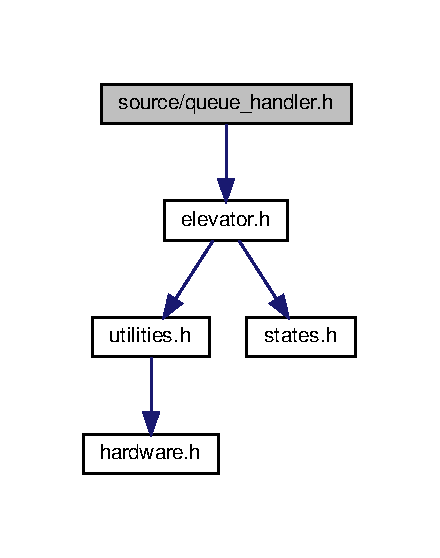
\includegraphics[width=272pt]{queue__handler_8h__incl}
\end{center}
\end{figure}
This graph shows which files directly or indirectly include this file\+:
\nopagebreak
\begin{figure}[H]
\begin{center}
\leavevmode
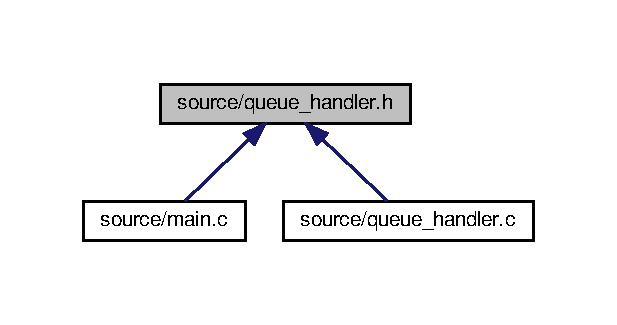
\includegraphics[width=350pt]{queue__handler_8h__dep__incl}
\end{center}
\end{figure}
\doxysubsection*{Macros}
\begin{DoxyCompactItemize}
\item 
\mbox{\Hypertarget{queue__handler_8h_a4774b0c12e9bdb975cdc19125b9343d5}\label{queue__handler_8h_a4774b0c12e9bdb975cdc19125b9343d5}} 
\#define {\bfseries QUEUE\+\_\+\+HANDLER\+\_\+\+NUMBER\+\_\+\+OF\+\_\+\+ROWS}~3
\end{DoxyCompactItemize}
\doxysubsection*{Functions}
\begin{DoxyCompactItemize}
\item 
void \mbox{\hyperlink{queue__handler_8h_a27e5de46fbd8cac82f06fc5e6b64f37e}{queue\+\_\+clear}} (\mbox{\hyperlink{structElevator}{Elevator}} $\ast$p\+\_\+elev)
\begin{DoxyCompactList}\small\item\em Sets all elements of queue\+\_\+matrix in an \mbox{\hyperlink{structElevator}{Elevator}} struct to zero. \end{DoxyCompactList}\item 
int \mbox{\hyperlink{queue__handler_8h_a6a8f2e61bafeaadb36377a3664a681e3}{queue\+\_\+get\+\_\+order}} (\mbox{\hyperlink{structElevator}{Elevator}} $\ast$p\+\_\+elev, \mbox{\hyperlink{hardware_8h_a796a8de8ce0ae769d7dbd3327a7bdbe7}{Hardware\+Order}} order\+\_\+type, int floor)
\begin{DoxyCompactList}\small\item\em Check a specified value in queue\+\_\+matrix in an \mbox{\hyperlink{structElevator}{Elevator}} struct. \end{DoxyCompactList}\item 
void \mbox{\hyperlink{queue__handler_8h_a3ce896fe20074af270bcbb349562dfd9}{queue\+\_\+set\+\_\+orders}} (\mbox{\hyperlink{structElevator}{Elevator}} $\ast$p\+\_\+elev)
\begin{DoxyCompactList}\small\item\em Updates queue\+\_\+matrix in an \mbox{\hyperlink{structElevator}{Elevator}} struct with new orders. \end{DoxyCompactList}\item 
void \mbox{\hyperlink{queue__handler_8h_a7b8d1f4f4b11dc91a3ed06449feea23d}{queue\+\_\+delete\+\_\+order}} (\mbox{\hyperlink{structElevator}{Elevator}} $\ast$p\+\_\+elev, \mbox{\hyperlink{hardware_8h_a796a8de8ce0ae769d7dbd3327a7bdbe7}{Hardware\+Order}} order\+\_\+type, int floor)
\begin{DoxyCompactList}\small\item\em Sets a value specified by {\ttfamily order\+\_\+type} and {\ttfamily floor} in the queue\+\_\+matrix in {\ttfamily p\+\_\+elev} to zero. \end{DoxyCompactList}\item 
int \mbox{\hyperlink{queue__handler_8h_ac73d563781c8a925a2f48a0a0274013e}{queue\+\_\+active\+\_\+orders\+\_\+floor}} (\mbox{\hyperlink{structElevator}{Elevator}} $\ast$p\+\_\+elev, int floor)
\begin{DoxyCompactList}\small\item\em Checks {\ttfamily floor} for any unhandled orders. \end{DoxyCompactList}\item 
int \mbox{\hyperlink{queue__handler_8h_a12d9773f1198f963edbd5cf50f177928}{queue\+\_\+active\+\_\+orders\+\_\+all\+\_\+floors}} (\mbox{\hyperlink{structElevator}{Elevator}} $\ast$p\+\_\+elev)
\begin{DoxyCompactList}\small\item\em Checks if there are any unhandled orders in {\ttfamily p\+\_\+elev}. \end{DoxyCompactList}\item 
\mbox{\hyperlink{hardware_8h_a2167c399a24df296afc432bcb88228af}{Hardware\+Movement}} \mbox{\hyperlink{queue__handler_8h_af977d3c209c783b26fe5fd385a7799f3}{queue\+\_\+get\+\_\+movement\+\_\+any\+\_\+direction}} (\mbox{\hyperlink{structElevator}{Elevator}} $\ast$p\+\_\+elev)
\begin{DoxyCompactList}\small\item\em Checks for the direction for the elevator to move, independent of order priorities. \end{DoxyCompactList}\item 
\mbox{\hyperlink{hardware_8h_a2167c399a24df296afc432bcb88228af}{Hardware\+Movement}} \mbox{\hyperlink{queue__handler_8h_a730a369784a44157f19c48e850068255}{queue\+\_\+get\+\_\+movement\+\_\+direction}} (\mbox{\hyperlink{structElevator}{Elevator}} $\ast$p\+\_\+elev)
\begin{DoxyCompactList}\small\item\em Checks for the direction for the elevator to move, with order priorities. If no priorities are found the function checks for directions for the elevator to move without order priorities. \end{DoxyCompactList}\item 
\mbox{\hyperlink{hardware_8h_a796a8de8ce0ae769d7dbd3327a7bdbe7}{Hardware\+Order}} \mbox{\hyperlink{queue__handler_8h_a5690c565e767b1bcdebb9c9a77d519e8}{queue\+\_\+get\+\_\+direction\+\_\+of\+\_\+order}} (\mbox{\hyperlink{structElevator}{Elevator}} $\ast$p\+\_\+elev)
\begin{DoxyCompactList}\small\item\em Checks the order type of the order just handled. \end{DoxyCompactList}\item 
int \mbox{\hyperlink{queue__handler_8h_a4d6b82c134f2aab959f52c4833b81d7d}{queue\+\_\+active\+\_\+orders\+\_\+in\+\_\+direction}} (\mbox{\hyperlink{structElevator}{Elevator}} $\ast$p\+\_\+elev, \mbox{\hyperlink{hardware_8h_a2167c399a24df296afc432bcb88228af}{Hardware\+Movement}} direction\+\_\+type)
\begin{DoxyCompactList}\small\item\em Searches for any unhandled orders at the floors in the direction which {\ttfamily direction\+\_\+type} specifies. \end{DoxyCompactList}\item 
int \mbox{\hyperlink{queue__handler_8h_a2a38a3e344c7c67f695b302b4de47697}{queue\+\_\+check\+\_\+orders\+\_\+current\+\_\+floor}} (\mbox{\hyperlink{structElevator}{Elevator}} $\ast$p\+\_\+elev)
\begin{DoxyCompactList}\small\item\em Checks if there are any orders at the current floor of {\ttfamily p\+\_\+elev} which are to be handled next. \end{DoxyCompactList}\end{DoxyCompactItemize}


\doxysubsection{Detailed Description}
Library for doing operations with a queue matrix defined in an \mbox{\hyperlink{structElevator}{Elevator}} struct. 



\doxysubsection{Function Documentation}
\mbox{\Hypertarget{queue__handler_8h_a12d9773f1198f963edbd5cf50f177928}\label{queue__handler_8h_a12d9773f1198f963edbd5cf50f177928}} 
\index{queue\_handler.h@{queue\_handler.h}!queue\_active\_orders\_all\_floors@{queue\_active\_orders\_all\_floors}}
\index{queue\_active\_orders\_all\_floors@{queue\_active\_orders\_all\_floors}!queue\_handler.h@{queue\_handler.h}}
\doxysubsubsection{\texorpdfstring{queue\_active\_orders\_all\_floors()}{queue\_active\_orders\_all\_floors()}}
{\footnotesize\ttfamily int queue\+\_\+active\+\_\+orders\+\_\+all\+\_\+floors (\begin{DoxyParamCaption}\item[{\mbox{\hyperlink{structElevator}{Elevator}} $\ast$}]{p\+\_\+elev }\end{DoxyParamCaption})}



Checks if there are any unhandled orders in {\ttfamily p\+\_\+elev}. 


\begin{DoxyParams}[1]{Parameters}
\mbox{\texttt{ in}}  & {\em p\+\_\+elev} & Pointer to an \mbox{\hyperlink{structElevator}{Elevator}} struct\\
\hline
\end{DoxyParams}
\begin{DoxyReturn}{Returns}
1 if there are any unhandled orders for {\ttfamily p\+\_\+elev} 
\end{DoxyReturn}


Definition at line 36 of file queue\+\_\+handler.\+c.

\mbox{\Hypertarget{queue__handler_8h_ac73d563781c8a925a2f48a0a0274013e}\label{queue__handler_8h_ac73d563781c8a925a2f48a0a0274013e}} 
\index{queue\_handler.h@{queue\_handler.h}!queue\_active\_orders\_floor@{queue\_active\_orders\_floor}}
\index{queue\_active\_orders\_floor@{queue\_active\_orders\_floor}!queue\_handler.h@{queue\_handler.h}}
\doxysubsubsection{\texorpdfstring{queue\_active\_orders\_floor()}{queue\_active\_orders\_floor()}}
{\footnotesize\ttfamily int queue\+\_\+active\+\_\+orders\+\_\+floor (\begin{DoxyParamCaption}\item[{\mbox{\hyperlink{structElevator}{Elevator}} $\ast$}]{p\+\_\+elev,  }\item[{int}]{floor }\end{DoxyParamCaption})}



Checks {\ttfamily floor} for any unhandled orders. 


\begin{DoxyParams}[1]{Parameters}
\mbox{\texttt{ in}}  & {\em p\+\_\+elev} & Pointer to an \mbox{\hyperlink{structElevator}{Elevator}} struct \\
\hline
\mbox{\texttt{ in}}  & {\em floor} & The floor to check\\
\hline
\end{DoxyParams}
\begin{DoxyReturn}{Returns}
1 if there are any unhandled orders at {\ttfamily floor} for {\ttfamily p\+\_\+elev}, 0 otherwise 
\end{DoxyReturn}


Definition at line 29 of file queue\+\_\+handler.\+c.

\mbox{\Hypertarget{queue__handler_8h_a4d6b82c134f2aab959f52c4833b81d7d}\label{queue__handler_8h_a4d6b82c134f2aab959f52c4833b81d7d}} 
\index{queue\_handler.h@{queue\_handler.h}!queue\_active\_orders\_in\_direction@{queue\_active\_orders\_in\_direction}}
\index{queue\_active\_orders\_in\_direction@{queue\_active\_orders\_in\_direction}!queue\_handler.h@{queue\_handler.h}}
\doxysubsubsection{\texorpdfstring{queue\_active\_orders\_in\_direction()}{queue\_active\_orders\_in\_direction()}}
{\footnotesize\ttfamily int queue\+\_\+active\+\_\+orders\+\_\+in\+\_\+direction (\begin{DoxyParamCaption}\item[{\mbox{\hyperlink{structElevator}{Elevator}} $\ast$}]{p\+\_\+elev,  }\item[{\mbox{\hyperlink{hardware_8h_a2167c399a24df296afc432bcb88228af}{Hardware\+Movement}}}]{direction\+\_\+type }\end{DoxyParamCaption})}



Searches for any unhandled orders at the floors in the direction which {\ttfamily direction\+\_\+type} specifies. 


\begin{DoxyParams}[1]{Parameters}
\mbox{\texttt{ in}}  & {\em p\+\_\+elev} & Pointer to an \mbox{\hyperlink{structElevator}{Elevator}} struct \\
\hline
\mbox{\texttt{ in}}  & {\em direction\+\_\+type} & Direction that the search for orders should be done in\\
\hline
\end{DoxyParams}
\begin{DoxyReturn}{Returns}
1 if there are unhandled orders for {\ttfamily p\+\_\+elev} in the direction of {\ttfamily direction\+\_\+type}, 0 otherwise 
\end{DoxyReturn}


Definition at line 97 of file queue\+\_\+handler.\+c.

\mbox{\Hypertarget{queue__handler_8h_a2a38a3e344c7c67f695b302b4de47697}\label{queue__handler_8h_a2a38a3e344c7c67f695b302b4de47697}} 
\index{queue\_handler.h@{queue\_handler.h}!queue\_check\_orders\_current\_floor@{queue\_check\_orders\_current\_floor}}
\index{queue\_check\_orders\_current\_floor@{queue\_check\_orders\_current\_floor}!queue\_handler.h@{queue\_handler.h}}
\doxysubsubsection{\texorpdfstring{queue\_check\_orders\_current\_floor()}{queue\_check\_orders\_current\_floor()}}
{\footnotesize\ttfamily int queue\+\_\+check\+\_\+orders\+\_\+current\+\_\+floor (\begin{DoxyParamCaption}\item[{\mbox{\hyperlink{structElevator}{Elevator}} $\ast$}]{p\+\_\+elev }\end{DoxyParamCaption})}



Checks if there are any orders at the current floor of {\ttfamily p\+\_\+elev} which are to be handled next. 


\begin{DoxyParams}[1]{Parameters}
\mbox{\texttt{ in}}  & {\em p\+\_\+elev} & Pointer to an \mbox{\hyperlink{structElevator}{Elevator}} struct\\
\hline
\end{DoxyParams}
\begin{DoxyReturn}{Returns}
1 if there are orders to handle next at current floor of {\ttfamily p\+\_\+elev} , 0 otherwise 
\end{DoxyReturn}


Definition at line 119 of file queue\+\_\+handler.\+c.

\mbox{\Hypertarget{queue__handler_8h_a27e5de46fbd8cac82f06fc5e6b64f37e}\label{queue__handler_8h_a27e5de46fbd8cac82f06fc5e6b64f37e}} 
\index{queue\_handler.h@{queue\_handler.h}!queue\_clear@{queue\_clear}}
\index{queue\_clear@{queue\_clear}!queue\_handler.h@{queue\_handler.h}}
\doxysubsubsection{\texorpdfstring{queue\_clear()}{queue\_clear()}}
{\footnotesize\ttfamily void queue\+\_\+clear (\begin{DoxyParamCaption}\item[{\mbox{\hyperlink{structElevator}{Elevator}} $\ast$}]{p\+\_\+elev }\end{DoxyParamCaption})}



Sets all elements of queue\+\_\+matrix in an \mbox{\hyperlink{structElevator}{Elevator}} struct to zero. 


\begin{DoxyParams}[1]{Parameters}
\mbox{\texttt{ out}}  & {\em p\+\_\+elev} & Pointer to an \mbox{\hyperlink{structElevator}{Elevator}} struct \\
\hline
\end{DoxyParams}


Definition at line 3 of file queue\+\_\+handler.\+c.

\mbox{\Hypertarget{queue__handler_8h_a7b8d1f4f4b11dc91a3ed06449feea23d}\label{queue__handler_8h_a7b8d1f4f4b11dc91a3ed06449feea23d}} 
\index{queue\_handler.h@{queue\_handler.h}!queue\_delete\_order@{queue\_delete\_order}}
\index{queue\_delete\_order@{queue\_delete\_order}!queue\_handler.h@{queue\_handler.h}}
\doxysubsubsection{\texorpdfstring{queue\_delete\_order()}{queue\_delete\_order()}}
{\footnotesize\ttfamily void queue\+\_\+delete\+\_\+order (\begin{DoxyParamCaption}\item[{\mbox{\hyperlink{structElevator}{Elevator}} $\ast$}]{p\+\_\+elev,  }\item[{\mbox{\hyperlink{hardware_8h_a796a8de8ce0ae769d7dbd3327a7bdbe7}{Hardware\+Order}}}]{order\+\_\+type,  }\item[{int}]{floor }\end{DoxyParamCaption})}



Sets a value specified by {\ttfamily order\+\_\+type} and {\ttfamily floor} in the queue\+\_\+matrix in {\ttfamily p\+\_\+elev} to zero. 


\begin{DoxyParams}[1]{Parameters}
\mbox{\texttt{ out}}  & {\em p\+\_\+elev} & Pointer to an \mbox{\hyperlink{structElevator}{Elevator}} struct \\
\hline
\mbox{\texttt{ in}}  & {\em order\+\_\+type} & The order type specified \\
\hline
\mbox{\texttt{ in}}  & {\em floor} & The floor specified \\
\hline
\end{DoxyParams}


Definition at line 25 of file queue\+\_\+handler.\+c.

\mbox{\Hypertarget{queue__handler_8h_a5690c565e767b1bcdebb9c9a77d519e8}\label{queue__handler_8h_a5690c565e767b1bcdebb9c9a77d519e8}} 
\index{queue\_handler.h@{queue\_handler.h}!queue\_get\_direction\_of\_order@{queue\_get\_direction\_of\_order}}
\index{queue\_get\_direction\_of\_order@{queue\_get\_direction\_of\_order}!queue\_handler.h@{queue\_handler.h}}
\doxysubsubsection{\texorpdfstring{queue\_get\_direction\_of\_order()}{queue\_get\_direction\_of\_order()}}
{\footnotesize\ttfamily \mbox{\hyperlink{hardware_8h_a796a8de8ce0ae769d7dbd3327a7bdbe7}{Hardware\+Order}} queue\+\_\+get\+\_\+direction\+\_\+of\+\_\+order (\begin{DoxyParamCaption}\item[{\mbox{\hyperlink{structElevator}{Elevator}} $\ast$}]{p\+\_\+elev }\end{DoxyParamCaption})}



Checks the order type of the order just handled. 


\begin{DoxyParams}[1]{Parameters}
\mbox{\texttt{ in}}  & {\em p\+\_\+elev} & Pointer an \mbox{\hyperlink{structElevator}{Elevator}} struct\\
\hline
\end{DoxyParams}
\begin{DoxyReturn}{Returns}
Order type of the order which {\ttfamily p\+\_\+elev} just handled 
\end{DoxyReturn}


Definition at line 89 of file queue\+\_\+handler.\+c.

\mbox{\Hypertarget{queue__handler_8h_af977d3c209c783b26fe5fd385a7799f3}\label{queue__handler_8h_af977d3c209c783b26fe5fd385a7799f3}} 
\index{queue\_handler.h@{queue\_handler.h}!queue\_get\_movement\_any\_direction@{queue\_get\_movement\_any\_direction}}
\index{queue\_get\_movement\_any\_direction@{queue\_get\_movement\_any\_direction}!queue\_handler.h@{queue\_handler.h}}
\doxysubsubsection{\texorpdfstring{queue\_get\_movement\_any\_direction()}{queue\_get\_movement\_any\_direction()}}
{\footnotesize\ttfamily \mbox{\hyperlink{hardware_8h_a2167c399a24df296afc432bcb88228af}{Hardware\+Movement}} queue\+\_\+get\+\_\+movement\+\_\+any\+\_\+direction (\begin{DoxyParamCaption}\item[{\mbox{\hyperlink{structElevator}{Elevator}} $\ast$}]{p\+\_\+elev }\end{DoxyParamCaption})}



Checks for the direction for the elevator to move, independent of order priorities. 


\begin{DoxyParams}[1]{Parameters}
\mbox{\texttt{ in}}  & {\em p\+\_\+elev} & Pointer to an \mbox{\hyperlink{structElevator}{Elevator}} struct\\
\hline
\end{DoxyParams}
\begin{DoxyReturn}{Returns}
Direction for the elevator {\ttfamily p\+\_\+elev} to move without order priorities 
\end{DoxyReturn}


Definition at line 43 of file queue\+\_\+handler.\+c.

\mbox{\Hypertarget{queue__handler_8h_a730a369784a44157f19c48e850068255}\label{queue__handler_8h_a730a369784a44157f19c48e850068255}} 
\index{queue\_handler.h@{queue\_handler.h}!queue\_get\_movement\_direction@{queue\_get\_movement\_direction}}
\index{queue\_get\_movement\_direction@{queue\_get\_movement\_direction}!queue\_handler.h@{queue\_handler.h}}
\doxysubsubsection{\texorpdfstring{queue\_get\_movement\_direction()}{queue\_get\_movement\_direction()}}
{\footnotesize\ttfamily \mbox{\hyperlink{hardware_8h_a2167c399a24df296afc432bcb88228af}{Hardware\+Movement}} queue\+\_\+get\+\_\+movement\+\_\+direction (\begin{DoxyParamCaption}\item[{\mbox{\hyperlink{structElevator}{Elevator}} $\ast$}]{p\+\_\+elev }\end{DoxyParamCaption})}



Checks for the direction for the elevator to move, with order priorities. If no priorities are found the function checks for directions for the elevator to move without order priorities. 


\begin{DoxyParams}[1]{Parameters}
\mbox{\texttt{ in}}  & {\em p\+\_\+elev} & Pointer to an \mbox{\hyperlink{structElevator}{Elevator}} struct\\
\hline
\end{DoxyParams}
\begin{DoxyReturn}{Returns}
Direction for {\ttfamily p\+\_\+elev} to move 
\end{DoxyReturn}


Definition at line 60 of file queue\+\_\+handler.\+c.

\mbox{\Hypertarget{queue__handler_8h_a6a8f2e61bafeaadb36377a3664a681e3}\label{queue__handler_8h_a6a8f2e61bafeaadb36377a3664a681e3}} 
\index{queue\_handler.h@{queue\_handler.h}!queue\_get\_order@{queue\_get\_order}}
\index{queue\_get\_order@{queue\_get\_order}!queue\_handler.h@{queue\_handler.h}}
\doxysubsubsection{\texorpdfstring{queue\_get\_order()}{queue\_get\_order()}}
{\footnotesize\ttfamily int queue\+\_\+get\+\_\+order (\begin{DoxyParamCaption}\item[{\mbox{\hyperlink{structElevator}{Elevator}} $\ast$}]{p\+\_\+elev,  }\item[{\mbox{\hyperlink{hardware_8h_a796a8de8ce0ae769d7dbd3327a7bdbe7}{Hardware\+Order}}}]{order\+\_\+type,  }\item[{int}]{floor }\end{DoxyParamCaption})}



Check a specified value in queue\+\_\+matrix in an \mbox{\hyperlink{structElevator}{Elevator}} struct. 


\begin{DoxyParams}[1]{Parameters}
\mbox{\texttt{ in}}  & {\em p\+\_\+elev} & Pointer to an \mbox{\hyperlink{structElevator}{Elevator}} struct \\
\hline
\mbox{\texttt{ in}}  & {\em order\+\_\+type} & The order type to check \\
\hline
\mbox{\texttt{ in}}  & {\em floor} & The floor to check\\
\hline
\end{DoxyParams}
\begin{DoxyReturn}{Returns}
1 if there is an unhandled order at {\ttfamily floor} with {\ttfamily order\+\_\+type} in {\ttfamily p\+\_\+elev}, 0 otherwise 
\end{DoxyReturn}


Definition at line 11 of file queue\+\_\+handler.\+c.

\mbox{\Hypertarget{queue__handler_8h_a3ce896fe20074af270bcbb349562dfd9}\label{queue__handler_8h_a3ce896fe20074af270bcbb349562dfd9}} 
\index{queue\_handler.h@{queue\_handler.h}!queue\_set\_orders@{queue\_set\_orders}}
\index{queue\_set\_orders@{queue\_set\_orders}!queue\_handler.h@{queue\_handler.h}}
\doxysubsubsection{\texorpdfstring{queue\_set\_orders()}{queue\_set\_orders()}}
{\footnotesize\ttfamily void queue\+\_\+set\+\_\+orders (\begin{DoxyParamCaption}\item[{\mbox{\hyperlink{structElevator}{Elevator}} $\ast$}]{p\+\_\+elev }\end{DoxyParamCaption})}



Updates queue\+\_\+matrix in an \mbox{\hyperlink{structElevator}{Elevator}} struct with new orders. 


\begin{DoxyParams}[1]{Parameters}
\mbox{\texttt{ out}}  & {\em p\+\_\+elev} & Pointer to an \mbox{\hyperlink{structElevator}{Elevator}} struct \\
\hline
\end{DoxyParams}


Definition at line 15 of file queue\+\_\+handler.\+c.


\hypertarget{states_8h}{}\section{source/states.h File Reference}
\label{states_8h}\index{source/states.\+h@{source/states.\+h}}


Library containing the state enum.  


This graph shows which files directly or indirectly include this file\+:
\nopagebreak
\begin{figure}[H]
\begin{center}
\leavevmode
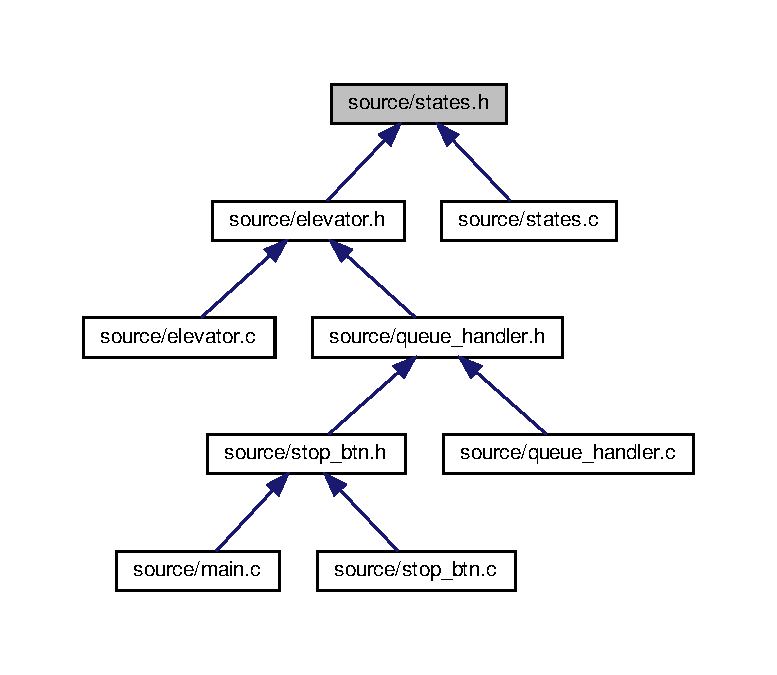
\includegraphics[width=350pt]{states_8h__dep__incl}
\end{center}
\end{figure}
\subsection*{Typedefs}
\begin{DoxyCompactItemize}
\item 
\mbox{\Hypertarget{states_8h_a9f34354b149588b399cf9448e20069be}\label{states_8h_a9f34354b149588b399cf9448e20069be}} 
typedef enum state {\bfseries state}
\end{DoxyCompactItemize}
\subsection*{Enumerations}
\begin{DoxyCompactItemize}
\item 
\mbox{\Hypertarget{states_8h_adc6e5733fc3c22f0a7b2914188c49c90}\label{states_8h_adc6e5733fc3c22f0a7b2914188c49c90}} 
enum {\bfseries state} \{ \newline
{\bfseries I\+N\+IT}, 
{\bfseries I\+D\+L\+E\+\_\+\+I\+N\+\_\+\+F\+L\+O\+OR}, 
{\bfseries I\+D\+L\+E\+\_\+\+I\+N\+\_\+\+S\+H\+A\+FT}, 
{\bfseries M\+O\+V\+E\+M\+E\+NT}, 
\newline
{\bfseries D\+O\+O\+R\+\_\+\+O\+P\+EN}, 
{\bfseries T\+I\+M\+ER}, 
{\bfseries S\+T\+O\+P\+\_\+\+B\+T\+N\+\_\+\+S\+H\+A\+FT}, 
{\bfseries S\+T\+O\+P\+\_\+\+B\+T\+N\+\_\+\+F\+L\+O\+OR}
 \}
\end{DoxyCompactItemize}


\subsection{Detailed Description}
Library containing the state enum. 


\hypertarget{timer_8h}{}\section{source/timer.h File Reference}
\label{timer_8h}\index{source/timer.\+h@{source/timer.\+h}}


Library for timer operations.  


{\ttfamily \#include $<$time.\+h$>$}\newline
Include dependency graph for timer.\+h\+:
\nopagebreak
\begin{figure}[H]
\begin{center}
\leavevmode
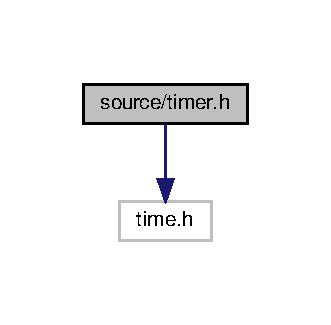
\includegraphics[width=159pt]{timer_8h__incl}
\end{center}
\end{figure}
This graph shows which files directly or indirectly include this file\+:
\nopagebreak
\begin{figure}[H]
\begin{center}
\leavevmode
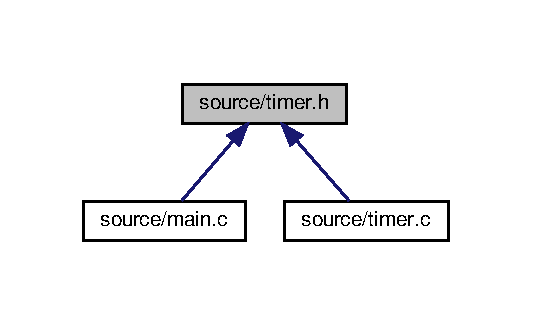
\includegraphics[width=256pt]{timer_8h__dep__incl}
\end{center}
\end{figure}
\subsection*{Functions}
\begin{DoxyCompactItemize}
\item 
clock\+\_\+t \hyperlink{timer_8h_a0359c2b3cbb84cd21b538f87732273f1}{timer\+\_\+set} ()
\begin{DoxyCompactList}\small\item\em Starts a timer. \end{DoxyCompactList}\item 
int \hyperlink{timer_8h_aa41d4f0fad92c3b70a923c2a37cc0cf2}{timer\+\_\+finished} (clock\+\_\+t previous\+\_\+time, int timer\+\_\+length\+\_\+ms)
\begin{DoxyCompactList}\small\item\em Checks if the timer has surpassed {\ttfamily timer\+\_\+length\+\_\+ms}. \end{DoxyCompactList}\end{DoxyCompactItemize}


\subsection{Detailed Description}
Library for timer operations. 



\subsection{Function Documentation}
\mbox{\Hypertarget{timer_8h_aa41d4f0fad92c3b70a923c2a37cc0cf2}\label{timer_8h_aa41d4f0fad92c3b70a923c2a37cc0cf2}} 
\index{timer.\+h@{timer.\+h}!timer\+\_\+finished@{timer\+\_\+finished}}
\index{timer\+\_\+finished@{timer\+\_\+finished}!timer.\+h@{timer.\+h}}
\subsubsection{\texorpdfstring{timer\+\_\+finished()}{timer\_finished()}}
{\footnotesize\ttfamily int timer\+\_\+finished (\begin{DoxyParamCaption}\item[{clock\+\_\+t}]{previous\+\_\+time,  }\item[{int}]{timer\+\_\+length\+\_\+ms }\end{DoxyParamCaption})}



Checks if the timer has surpassed {\ttfamily timer\+\_\+length\+\_\+ms}. 


\begin{DoxyParams}[1]{Parameters}
\mbox{\tt in}  & {\em previous\+\_\+time} & Reference time to compare current time with \\
\hline
\mbox{\tt in}  & {\em timer\+\_\+length\+\_\+ms} & Timer length in milliseconds \\
\hline
\end{DoxyParams}
\begin{DoxyReturn}{Returns}
1 if the timer is greater than {\ttfamily timer\+\_\+length\+\_\+ms}, 0 otherwise 
\end{DoxyReturn}


Definition at line 7 of file timer.\+c.

\mbox{\Hypertarget{timer_8h_a0359c2b3cbb84cd21b538f87732273f1}\label{timer_8h_a0359c2b3cbb84cd21b538f87732273f1}} 
\index{timer.\+h@{timer.\+h}!timer\+\_\+set@{timer\+\_\+set}}
\index{timer\+\_\+set@{timer\+\_\+set}!timer.\+h@{timer.\+h}}
\subsubsection{\texorpdfstring{timer\+\_\+set()}{timer\_set()}}
{\footnotesize\ttfamily clock\+\_\+t timer\+\_\+set (\begin{DoxyParamCaption}{ }\end{DoxyParamCaption})}



Starts a timer. 

\begin{DoxyReturn}{Returns}
Time used by the program so far (user time + system time) 
\end{DoxyReturn}


Definition at line 3 of file timer.\+c.


\hypertarget{utilities_8h}{}\section{source/utilities.h File Reference}
\label{utilities_8h}\index{source/utilities.\+h@{source/utilities.\+h}}


Useful functions.  


{\ttfamily \#include \char`\"{}hardware.\+h\char`\"{}}\newline
Include dependency graph for utilities.\+h\+:\nopagebreak
\begin{figure}[H]
\begin{center}
\leavevmode
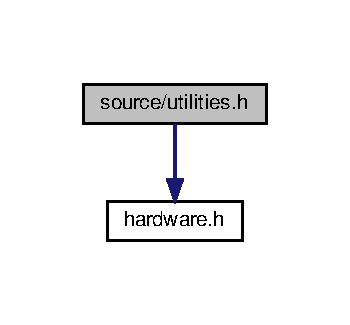
\includegraphics[width=168pt]{utilities_8h__incl}
\end{center}
\end{figure}
This graph shows which files directly or indirectly include this file\+:
\nopagebreak
\begin{figure}[H]
\begin{center}
\leavevmode
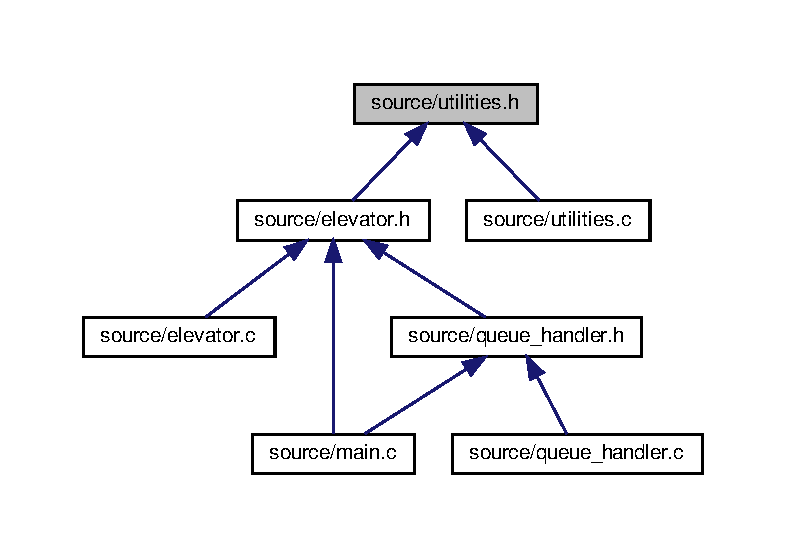
\includegraphics[width=350pt]{utilities_8h__dep__incl}
\end{center}
\end{figure}
\subsection*{Functions}
\begin{DoxyCompactItemize}
\item 
int \hyperlink{utilities_8h_aa73c7e63d6b2dac6a0e545da4098f412}{read\+\_\+all\+\_\+floor\+\_\+sensors} ()
\begin{DoxyCompactList}\small\item\em Reads all 4 floor sensors. \end{DoxyCompactList}\item 
\hyperlink{hardware_8h_a2167c399a24df296afc432bcb88228af}{Hardware\+Movement} \hyperlink{utilities_8h_a4240666d5d1f83f5ef5d3dc8cab8f339}{opposite\+\_\+direction} (\hyperlink{hardware_8h_a2167c399a24df296afc432bcb88228af}{Hardware\+Movement} direction)
\begin{DoxyCompactList}\small\item\em Used for getting the opposite direction of {\ttfamily direction}. \end{DoxyCompactList}\end{DoxyCompactItemize}


\subsection{Detailed Description}
Useful functions. 



\subsection{Function Documentation}
\mbox{\Hypertarget{utilities_8h_a4240666d5d1f83f5ef5d3dc8cab8f339}\label{utilities_8h_a4240666d5d1f83f5ef5d3dc8cab8f339}} 
\index{utilities.\+h@{utilities.\+h}!opposite\+\_\+direction@{opposite\+\_\+direction}}
\index{opposite\+\_\+direction@{opposite\+\_\+direction}!utilities.\+h@{utilities.\+h}}
\subsubsection{\texorpdfstring{opposite\+\_\+direction()}{opposite\_direction()}}
{\footnotesize\ttfamily \hyperlink{hardware_8h_a2167c399a24df296afc432bcb88228af}{Hardware\+Movement} opposite\+\_\+direction (\begin{DoxyParamCaption}\item[{\hyperlink{hardware_8h_a2167c399a24df296afc432bcb88228af}{Hardware\+Movement}}]{direction }\end{DoxyParamCaption})}



Used for getting the opposite direction of {\ttfamily direction}. 


\begin{DoxyParams}[1]{Parameters}
\mbox{\tt in}  & {\em direction} & Input direction \\
\hline
\end{DoxyParams}
\begin{DoxyReturn}{Returns}
Opposite direction of {\ttfamily direction} 
\end{DoxyReturn}


Definition at line 11 of file utilities.\+c.

\mbox{\Hypertarget{utilities_8h_aa73c7e63d6b2dac6a0e545da4098f412}\label{utilities_8h_aa73c7e63d6b2dac6a0e545da4098f412}} 
\index{utilities.\+h@{utilities.\+h}!read\+\_\+all\+\_\+floor\+\_\+sensors@{read\+\_\+all\+\_\+floor\+\_\+sensors}}
\index{read\+\_\+all\+\_\+floor\+\_\+sensors@{read\+\_\+all\+\_\+floor\+\_\+sensors}!utilities.\+h@{utilities.\+h}}
\subsubsection{\texorpdfstring{read\+\_\+all\+\_\+floor\+\_\+sensors()}{read\_all\_floor\_sensors()}}
{\footnotesize\ttfamily int read\+\_\+all\+\_\+floor\+\_\+sensors (\begin{DoxyParamCaption}{ }\end{DoxyParamCaption})}



Reads all 4 floor sensors. 

\begin{DoxyReturn}{Returns}
Current floor if elevator is in a floor, -\/1 if elevator is in the shaft, i.\+e none of the sensors are triggered 
\end{DoxyReturn}


Definition at line 3 of file utilities.\+c.


%--- End generated contents ---

% Index
\backmatter
\newpage
\phantomsection
\clearemptydoublepage
\addcontentsline{toc}{chapter}{Index}
\printindex

\end{document}
